
%!TEX root = main.tex

\section{Notation}

\begin{itemize}
	\item $\RV{X}$ is a random variable, $X$ is its codomain and $\sigalg{X}$ is the $\sigma$-algebra on $X$
	\item Bold letters $\prodSet{X}$ may be used for product spaces, $\vecVal{x}$ for elements of product spaces, $\mathbf{f}$ for vector valued functions and $\vecRV{X}$ for random variables taking values in product spaces. The absence of bold font does not imply the absence of product space structure
	\item Nodes in a graph are italic sans serif $\nod{X}$
	\item Given an indexed product space $\prod_{i\in \indx{I}} X_i$, $\pi_i:\prod_{i\in \indx{I}} X_i\to X_i$ is the projection map $(x_1,...,x_i,...,x_n)\mapsto x_i$
	\item Given a product space $X\times Y$, $\pi_X:X\times Y\to X$ is the projection map $(x,y)\mapsto x$
	\item Given an index set $\indx{I}$, $\prodSet{X}_{\indx{I}}$ is the indexed product space $\prod_{i\in \indx{I}} X_i$
	\item $[n]$ is the index set $\{1,...,n\}$ for $n\in\mathbb{N}$
	\item Given an indexed product space $\prodSet{X}_{[n]}$, $\prodSet{X}_{<j}$ is the set $\prod_{i=1}^j X_i$
	\item $\utimes$ is the coupled tensor product, see Definition \ref{def:ctensor}
	\item Given a random variable $\RV{X}$, $F_{\RV{X}}$ is the associated Markov kernel, see Definition \ref{def:functional_kernel}
	\item See section \ref{sssec:string_diagram_manipulation} for rules of string diagram manipulation
	\item $\stopper{0.2}_X:X\to \Delta(\{*\})$ is the discard map defined in Equation \ref{eq:discard}
\end{itemize}

\section{What is the difference between Causal Bayesian Networks and See-Do models?}

See-Do models and Causal Bayesian Networks (and related models such as SCMs) are quite different in their appearance and in the interpretation of various elements. In defining See-Do models, we assume that there is a decision problem that fixes in advance the observation space $E$, the space of consequences $F$ and the set of available decisions $D$. By including $D$, See-Do models have an agent ``baked in'' to the definition. In contrast, Causal Bayesian Networks assume that a set of observed variables $\mathbf{X}$ and a set of unobserved variables $\mathbf{U}$ is fixed by nature. A subtlety here is that $\mathbf{U}$ is generally \emph{not} known, but it may be assumed that whatever variables actually comprise $\mathbf{U}$, they may be generically representable by some known set of variables $\mathbf{U}'$ without loss. Because a set of decisions $D$ is absent, Causal Bayesian Networks appear to model agent-independent ``causal relationships''.

Despite the fact that Causal Bayesian Networks don't seem to built to model the consequences of an agent's decision making, they are nonetheless considered to be appropriate for this purpose. This is because the ``do-operations'' that Causal Bayesian Networks support are considered to have some relationship to any set $D$ decisions some agent might want to consider.

The question of how this relationship might be determined in general is one that I have not seen addressed anywhere. Typically, the approach taken is ``I know it when I see it''. For example, if I were a doctor and I could either A) hand a patient a prescription or B) not hand the patient the prescription, and if I had a set of observational data of past patients including a variable $\RV{S}$ representing whether or not they had received a prescription for the drug, I could consider option A to correspond to $do(\RV{S}=1)$ and option B to correspond to $do(\RV{S}=0)$ in some causal model (perhaps in the ``true'' causal model). While this might appear to be reasonable, we should be cautious: this is a completely \emph{ad-hoc} assumption.

In fact, given a sufficiently rich set of variables $\mathbf{U}\cup\RV{X}$, I argue that $do(\RV{S})$ will almost never even approximate the consequences of an action known in advance to fix the value of some variable $\RV{S}$. For this reason, it is valuable to have a theory like CSDT that is concerned only with the consequences of actions.

\subsection{Influence Diagrams vs See-Do models}

Influence diagrams are used to represent causal models in a manner similar to, but not quite the same as, Causal Bayesian Networks. Using the version found in \citet{dawid_influence_2002}, an influence diagram is a directed acyclic graph (DAG) with two node types: ``chance'' nodes and ``decision'' nodes. For example:

\begin{align}
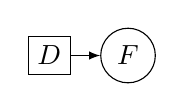
\begin{tikzpicture}[scale = 2]
\path (0,0) node[rectangle,draw] (D) {$\nod{D}$}
++ (0.5,0) node[circle,draw] (F) {$\nod{F}$};
\draw[-latex] (D) -- (F);
\end{tikzpicture}\label{eq:simple_ID}
\end{align}

Is an influence diagram with the decision node $\nod{D}$ and the chance node $\nod{F}$. When nodes are associated with sets representing possible values, influence diagrams represent sets of Markov kernels. For example, if we associate the measurable set $(D,\mathcal{D})$ with $\nod{D}$ and $(F,\mathcal{F})$ with $\nod{F}$, then we could take Diagram \ref{eq:simple_ID} to represent the set of all Markov kernels $D\to \Delta(\mathcal{F})$, or if we add some additional assumptions it might represent a particular subset $S\subset \Delta(\mathcal{F})^D$ of these kernels that share certain properties. Compare this to a string diagram:

\begin{align}
\begin{tikzpicture}
\path (0,0) node (D) {$D$}
++ (0.7,0) node[kernel] (K) {$\kernl{K}$}
++ (0.7,0) node (F) {$F$};
\draw (D) -- (K) -- (F);
\end{tikzpicture}
\end{align}

This diagram represents a \emph{particular} Markov kernel $\kernl{K}:D\to \Delta(\mathcal{F})$. A set such as that represented by Diagram \ref{eq:simple_ID} could be constructed by creating a set $\Theta$ and a function $f:\Theta\to S$ that indexes each element of $S$ with $\theta\in \Theta$. Then $S=\{f(\theta)|\theta\in \Theta\}$. If $f$ is measurable then there is a Markov kernel $\kernl{T}:\Theta\times D\to \Delta(\mathcal{F})$ such that $f(\theta)=\kernl{T}_{\theta,\_}$\todo{notation}. In this sense, for any additional assumptions that are combined with Diagram \ref{eq:simple_ID} to yield the set $S$ of Markov kernels, there exists a single Markov kernel $\kernl{T}:\Theta\times D\to \Delta(\mathcal{F})$ that generates $S$. $\kernl{T}$ can be drawn as

\begin{align}
\begin{tikzpicture}
\path (0,0) node (D) {$D$}
+ (0,0.5) node (T) {$\Theta$}
++ (0.7,0.25) node[kernel] (K) {$\kernl{T}$}
++ (0.7,0) node (F) {$F$};
\draw (D) to [out=0,in=180] ($(K.west)+(0,-0.1)$) (K) -- (F);
\draw (T) to [out=0,in=180] ($(K.west) + (0,0.1)$);
\end{tikzpicture}\label{eq:simple_ID_kernel}
\end{align}

Diagram \ref{eq:simple_ID_kernel} has a few more elements that Diagram \ref{eq:simple_ID} - $\Theta$ and $\kernl{T}$ in particular. If I were to define exactly what $D$, $\Theta$, $\kernl{T}$ and $F$ were, Diagram \ref{eq:simple_ID_kernel} would represent a unique Markov kernel. On the other hand, Diagram \ref{eq:simple_ID} along with a precise definition of $D$ and $F$ could represent many different sets of Markov kernels, depending on whatever additional properties I want elements of $S$ to share. Loosely, we can say that for any kernel $\kernl{T}$, there is a diagram \ref{eq:simple_ID} along with additional assumptions that represents ``the same thing''\todo{Under the condition that the choice of index ``doesn't matter'' somehow}.

Influence diagrams \emph{as typically used in causal modelling} usually additional assumptions. For example, \citet{dawid_influence_2002} proposes that $D$ contains a special ``do nothing'' element $o\in D$ such that the observations in state $\theta$ are given by $\kernl{T}_{\theta,o}$\todo{notation} and consequences in state $\theta$ are given by $\kernl{T}_{\theta,\_}$. This corresponds to the See-Do model

\begin{align}
\begin{tikzpicture}
\path (0,0) node (D) {$D$}
+ (0,0.5) node (T) {$\Theta$}
+ (0.5,0.5) coordinate (copy0)
++ (1.5,0.25) node[kernel] (K) {$\kernl{T}$}
+ (0,0.5) node[kernel] (To) {$\kernl{T}_{\_,o}$}
++ (1,0) node (F) {$F$}
+(0,0.5) node (E) {$F$};
\draw (D) to [out=0,in=180] ($(K.west)+(0,-0.1)$) (K) -- (F);
\draw (T) -- (copy0) to [out=0,in=180] ($(K.west) + (0,0.1)$);
\draw (T) -- (copy0) to [out=0,in=180] (To) (To) -- (E);
\end{tikzpicture}
\end{align} 

While this is a feature of influence diagrams in \citet{dawid_influence_2002}, \emph{in general} a diagram like \ref{eq:simple_ID} can represent an arbitrary set of typed Markov kernels. See-Do models generate $\Theta$-indexed sets of Markov kernels. We can therefore represent generic See-Do models with influence diagrams.

\todo[inline]{There is some kind of measurability condition needed to make the two representations coincide}

Concretely, given the influence diagram
\begin{align}\label{eq:see_do_id}
\diagram{I} = 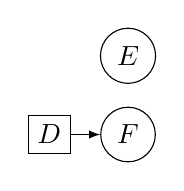
\begin{tikzpicture}[scale = 2]
\path (0,0) node[circle,draw] (E) {$\nod{E}$}
++ (-0.5,-0.5) node[rectangle,draw] (D) {$\nod{D}$}
++ (0.5,0) node[circle,draw] (F) {$\nod{F}$};
\draw[-latex] (D) -- (F);
\end{tikzpicture}
\end{align}

and any See-Do model $\kernl{T}:\Theta\times D\to \Delta(\mathcal{E}\otimes \mathcal{F})$ there exists a set of auxhiliary conditions $A$ such that the model $(\diagram{I},A)$ is equivalent to $\kernl{T}$\todo{subject to irrelevance of index $\Theta$}. To illustrate how influence diagrams and string diagrams compare, $\kernl{T}$ can be drawn:

\begin{align}
\kernl{T}:=\begin{tikzpicture}
\path (0,0) node (D) {$D$}
+ (0,0.5) node (T) {$\Theta$}
+ (0.5,0.5) coordinate (copy0)
++ (1.5,0.25) node[kernel] (K) {$\kernl{C}$}
+ (0,0.5) node[kernel] (To) {$\kernl{H}$}
++ (1,0) node (F) {$E$}
+(0,0.5) node (E) {$F$};
\draw (D) to [out=0,in=180] ($(K.west)+(0,-0.1)$) (K) -- (F);
\draw (T) -- (copy0) to [out=0,in=180] ($(K.west) + (0,0.1)$);
\draw (T) -- (copy0) to [out=0,in=180] (To) (To) -- (E);
\end{tikzpicture}
\end{align} 

\todo[inline]{Maybe move the following to an appendix?}

\begin{definition}[Markov kernel/influence diagram compatibility]
	Given a Markov kernel $\kernl{K}:E\to \Delta(\sigalg{F})$, an influence diagram $\diagram{I}=(S,A,E)$ and an injective $f:X\cup A\to\sigalg{F}\otimes\sigalg{E}$ which assigns each node to exactly one random variable in $\sigalg{F}\otimes\sigalg{E}$, if for all $X_1,X_2\in\prodSet{X}$ we have $\nod{X}_1\perp_{\diagram{I}} \nod{X}_2\implies f(\nod{X}_1) \CI_{K} f(\nod{X}_2)$ 
	\todo[inline]{still need to \emph{define} conditional independence WRT kernels, though I think I can do so}
\end{definition}

Consider an arbitrary See-Do model $\seedo:D\times \Theta\to \Delta(\sigalg{E}_1\otimes\sigalg{E}_2)$ and random variables $\RV{D}:=\pi_D,\RV{E}:=\pi_E,\RV{F}:=\pi_F$ on $\sigalg{D}\otimes\sigalg{E}\otimes\sigalg{F}$. For any $\theta\in \Theta$, $\seedo_\theta$ is compatible with the influence diagram $\diagram{I}=(\{\nod{E},\nod{F}\},\{\nod{D}\},\{\nod{D}\rightarrowtriangle \nod{F}\})$ with respect to the injective function
\begin{align}
	f:\begin{cases}&\nod{A}\mapsto \RV{D}\\
	&\nod{E}\mapsto \RV{E}\\
	&\nod{F}\mapsto \RV{F} \end{cases}
\end{align} 

There is always some $\kernl{H}:\Theta\to\Delta(\sigalg{E})$ and $\kernl{C}:\Theta\times D\to \Delta(\sigalg{E}\otimes\sigalg{F})$ such that: $\seedo_\theta$ is equal to
\begin{align}
	\seedo_\theta &= \begin{tikzpicture}[xscale=1.5]
	\path(0,0) node[kernel] (H) {$\kernl{H}_\theta$}
	+ (0.5,0) node (E) {$\RV{E}$}
	++ (-0.5,-0.5) node (D) {$\RV{D}$}
	++(0.5,0) node[kernel] (C) {$\kernl{C}_\theta$}
	++ (0.5,0) node (F) {$\RV{F}$};
	\draw (H) -- (E);
	\draw (D) -- (C) -- (F);
	\end{tikzpicture}
\end{align}

Which implies $\RV{E}\CI_{\seedo_\theta} \RV{F}$ and $\RV{E}\CI_{\seedo_\theta} \RV{D}$.

The influence diagram
\begin{align}\label{eq:see_do_id}
\diagram{I} = 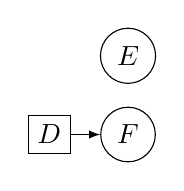
\begin{tikzpicture}[scale = 2]
\path (0,0) node[circle,draw] (E) {$\nod{E}$}
++ (-0.5,-0.5) node[rectangle,draw] (D) {$\nod{D}$}
++ (0.5,0) node[circle,draw] (F) {$\nod{F}$};
\draw[-latex] (D) -- (F);
\end{tikzpicture}
\end{align}

Features the d-separations $\nod{E}\perp_\diagram{I}\nod{F}$ and $\nod{E}\perp_\diagram{I}\nod{D}$\citep{peters_elements_2017,woodward_causation_2016,dawid_influence_2002}. Thus $\seedo_\theta$ is compatible with $\mathcal{I}$ for all $\theta\in\Theta$.

\subsection{Influence diagrams vs Causal Bayesian Networks}

See-Do models can always be represented by influence diagrams with auxhiliary assumptions. We can then learn something about how Causal Bayesian Networks compare to See-Do models by asking how they compare to influence diagrams. The key difference between Causal Bayesian Networks and influence diagrams is that the diagrams do not contain decision nodes. Instead of Diagram \ref{eq:simple_ID}, a Causal Bayesian Network for the same system might be

\begin{align}

\begin{tikzpicture}[scale = 2]
\path (0,0) node[circle,draw] (F) {$\nod{F}$};
\end{tikzpicture}\label{eq:simple_CBN}
\end{align}

The difference between Diagram \ref{eq:simple_ID} and Diagram \ref{eq:simple_CBN} is that the former demands a set $D$ to be bound to the decision node $\nod{D}$ and a set $F$ to be bound to $\nod{F}$, while Diagram \ref{eq:simple_CBN} demands only $F$. Instead of explicitly representing decisions that can be chosen, Causal Bayesian Networks \emph{by default} feature a set of \emph{do-interventions} on the chance nodes which seem to have a role similar to decisions in influence diagrams and See-Do models (in fact, \citet{pearl_causality:_2009} pg 108 suggests that do-interventions and decisions are the same thing). This default set of do-interventions is what allows CBNs to avoid explicitly requiring a set $D$. If a set of decisions is required that is not equivalent to the set of do-interventions, this can be specified via auxhiliary assumptions, although in practice influence diagrams are usually adopted such as in \citep{yang_characterizing_2018} \todo{some more examples}.

Dealing with a set of decisions $D$ can be troublesome. It can easily be the case that, for example, I might be tasked with inferring a consequence map that someone else might use and I am not privy to the decisions that they might be able to make. In this case, I'd need to pick a set of decisions $D$ which I am pretty sure covers all the possibilities. 

Alternatively, the set $D$ might be unworkably large. The set of \emph{all} the decisions you could in principle make at this moment in as much detail as you can - this is clearly something that's far too big to write down and work with in solving an inference problem.

Speculatively, the fact that Causal Bayesian Networks default to do-interventions might help with the problems of unknown or unworkably large decision sets. If any possible decision must be resolvable to do-interventions of some type, and the effects of do-interventions are well defined, then could provide a basis for partially solving \todo{as in, doing the inference but not picking the best option} decision problems while remaining ignorant of the particular set of decisions that will ultimately be selected from.

Beyond this, causal effects as they are informally understood \emph{seem} to refer to univeral things, not things that depend on the set of decisions one has available. While not an especially strong reason to avoid specifying $D$ in causal models, it is a reason nonetheless.

Do-interventions, however, cannot solve these problems. If there are no restrictions on the variables that may be included in a CBN model, then as we show do-operations and equation surgery frequently produce invalid results. To ensure that any do-interventions at all are well defined, Causal Bayesian Networks require the specification of ``intervenable variables'' or ``basic interventions'', a requirement that is analogous to the requirement of a set of decisions $D$ in See-Do models and influence diagrams. Specifying $D$ may be difficult, but the do-intervention paradigm provides no solutions to this difficulty; it merely sweeps it under the rug.

\subsection{What is meant by ``variables''?}


\todo[inline]{Not sure where to put it, but Pearl pp 162-163 puts his models on the hook for including arbitrary variables}


\subsection{Necessary relationships}

The relationship between a person's body mass index, their weight and their height defines what body mass index is. A fundamental claim of ours is that any causal model that defines ``the causal effect of body mass index'' should do so without reference to any submodel that violates this definitional relationship violation of the definition. This is an important assumption, and it rests on a judgement of what causal models ought to do. I think it is quite clear that when anyone asks for a causal effect, they expect that any operations required to define the causal effect \emph{do not change the definitions of the variables they are employing}. While theories of causality have a role in sharpening our understanding of the term \emph{causal effect}, the thing called a ``causal effect'' in an SCM should still respect some of our pre-theoretic intuitions about what causal effects are or else it should be called something else. ``Causal effects'' that depend on redefining variables do not respect pre-theoretic intuitions about what causal effects are:

\begin{itemize}
	\item If I ask for the ``causal effect of a person's BMI'', I do not imagine that I am asking what would happen if someone's BMI were defined to be something other than their weight divided by their height
	\item If I ask for the ``causal effect of a person's weight'', I do not imagine that I am asking what would happen if someone's weight were not equal to their volume multiplied by their density
	\item If I ask for the ``causal effect of a person's weight'', I also do not imagine that I am asking what would happen if their weight were not equal to the weight of fat in their body plus the weight of all non-fat parts of their body
	\item If I ask for the ``causal effect of taking a medicine'', I do not imagine that I am asking what would happen if a person were declared to have taken a medicine independently of whatever substances have actually entered their body and how they entered
\end{itemize}

We will call relationships that have to hold \emph{necessary relationships}. We provide the example of relationships that have to hold by definition as examples, but definitions may not be the only variety of necessary relationships. For example, one might also wish to stipulate that certain laws of physics are required to hold in all submodels.

If a causal model contains variables that are necessarily related, then an intervention on one of them must always change another variable in the relationship. If I change a person's weight, their height or BMI must change (or both). If I change their height, their weight or BMI must change and if I change their BMI then their weight or height must change. This conflicts with the usual acyclic definition of causal models, where the proposition that $\RV{A}$ causes $\RV{B}$ rules out the possibility that $\RV{B}$ or any of its descendents are a cause of $\RV{A}$. Thus in an acyclic model it isn't possible for for an intervention on BMI to change weight or height and interventions on weight and height to also change BMI. Theroem \ref{th:recursive_no_interventions} formalises this conflict for recursive structural causal models: for any set of variables that are necessarily related by a cyclic relationship, at least one of them has no hard interventions defined.

\subsection{Recursive Structural Causal Models}

We begin by showing that necessary relationships are incompatible with structural causal models.

\begin{definition}[Recursive Structural Causal Model]\label{def:acSCM}
A recursive structural causal model (SCM) is a tuple 
	\begin{align}
		\mathcal{M}:=\langle N,M,\prodSet{X}_{[N]},\mathbf{E}_{[M]},\{f_i|i\in[N]\},\mathbb{P}_{\mathcal{E}}\rangle
	\end{align}
	where 
	\begin{itemize}
		\item $N\in \mathbb{N}$ is the number of \emph{endogenous variables} in the model
		\item $M\in \mathbb{N}$ is the number of \emph{exogenous variables} in the model
		\item $\prodSet{X}_{[N]}:=\{X_i|i\in[N]\}$ where, for each $i\in [N]$, $(X_i,\mathcal{X}_i)$ is a standard measurable space taking and the codomain of the $i$-th endogenous variable
		\item $\mathbf{E}_{[M]}:=\{E_j|j\in[M]\}$ where, for $j\in [M]$, $E_j$ is a standard measurable space and the codomain of the $j$-th exogenous variable
		\item $f_i:\prodSet{X}_{<i}\times\mathbf{E}_{\indx{J}}\to X_i$ is a measurable function which we call \emph{the causal mechanism controlling the $i$-th endogenous variable}
		\item $\mathbb{P}_{\mathcal{E}}\in \Delta(\mathbf{E}_{\indx{J}})$ is a probability measure on the space of exogenous variables
	\end{itemize}
\end{definition}

\begin{definition}[Observable kernel]
Given an SCM $\mathcal{M}$ with causal mechanisms $\{f_i|i\in [N]\}$, define the \emph{observable kernel} $G_{i}:E\to \Delta(\prodSet{X}_{[i]})$ recursively:
\begin{align}
	G_1 &= \begin{tikzpicture}
	\path (0,0) node (E) {$\mathbf{E}_{[M]}$}
	++ (1,0) node[kernel] (F1) {$F_{f_1}$}
	++(1,0) node (X) {$X_1$};
	\draw (E) -- (F1) -- (X);
	\end{tikzpicture}f_1 \label{eq:gen_base}\\
	G_{n+1} &= \begin{tikzpicture}
	\path (0,0) node (E) {$\mathbf{E}_{[M]}$}
	++ (0.8,0) coordinate (copy0)
	++ (0.5,0) node[kernel] (Gn) {$G_{n}$}
	++ (0.5,0) coordinate (copy1)
	++ (0.7,0) coordinate (skip)
	+  (0,-0.5) node[kernel] (Fn) {$F_{f_{n+1}}$}
	++ (1.3,0) node (Xn) {$\prodSet{X}_{<{n+1}}$}
	+ (0,-0.5) node (Xn1) {$X_{n+1}$};
	\draw (E) -- (Gn) -- (Xn);
	\draw (copy0) to [bend right] ($(Fn.west) + (0,-0.15)$);
	\draw (copy1) to [bend right] ($(Fn.west) + (0,0.15)$);
	\draw (Fn) -- (Xn1);
	\end{tikzpicture}\label{eq:gen_step}
\end{align}
\end{definition}

\begin{definition}[Joint distribution on endogenous variables]
The \emph{joint distribution on endogenous variables} defined by $\mathcal{M}$ is $\mathbb{P}_{\mathcal{M}}:=\mathbb{P}_\mathcal{E} G_N$ (which is the regular kernel product, see Definition \ref{ssec:product_notation}). For each $i\in[N]$ define the random variable $\RV{X}_i:\prodSet{X}_{[N]}\to X_i$ as the projection map $\pi_i:(x_1,...,x_i,..,x_N)\mapsto x_i$. By Lemma \ref{lem:coupled_product_is_ident}, $\utimes_{i\in [N]} \RV{X}_i = \mathrm{Id}_{\prodSet{X}_{[N]}}$, and so $\mathbb{P}_{\mathcal{M}}$ is the joint distribution of the variables $\{\RV{X}_i|i\in[N]\}$.
\end{definition}

I use the notation $\mathbb{P}_{\mathcal{M}}$ rather than $\mathbb{P}_{\RV{X}_{[N]}}$ to emphasize the dependence on the model $\mathcal{M}$.

\begin{lemma}[Coupled product of all random variables is the identity]\label{lem:coupled_product_is_ident}
$\utimes_{i\in [N]} \RV{X}_i = \mathrm{Id}_{\prodSet{X}_{[N]}}$
\end{lemma}

\begin{proof}
for any $\prodSet{X}\in \prodSet{X}_{[N]}$,
\begin{align}
\utimes_{i\in [N]} \RV{X}_i (\prodSet{X}) &= (\pi_1(\prodSet{X}),...,\pi_N(\prodSet{X}))\\
	&= (x_1,...,x_n)\\
	&= \prodSet{X}
\end{align}
\end{proof}

\begin{definition}[Hard Interventions]
Let $\mathscr{M}$ be the set of all $SCMs$ sharing the indices, spaces and measure $\langle N,M,\prodSet{X}_{\indx{I}},\mathbf{E}_{[M]},\mathbb{P}_{\mathcal{E}}\rangle$. Note that the causal mechanisms are not fixed.

Given an SCM $\mathcal{M}=\langle N,M,\prodSet{X}_{\indx{I}},\mathbf{E}_{[M]},\{f_i|i\in[N]\},\mathbb{P}_{\mathcal{E}}\rangle$ and $\mathcal{S}\subset[N]$, a \emph{hard intervention} on $\RV{X}_\mathcal{S}$ is a map $Do_{\mathcal{S}}:\prodSet{X}_\mathcal{S}\times\mathscr{M}\to \mathscr{M}$ such that for $\mathbf{a}\in \prodSet{X}_S$, $Do_{\mathcal{S}}(\mathbf{a},\mathcal{M}) = \langle N,M,\prodSet{X}_{\indx{I}},\mathbf{E}_{[M]},\{f'_i|i\in[N]\},\mathbb{P}_{\mathcal{E}}\rangle$ where
\begin{align}
	f_i' &= f_i  &i\not\in \mathcal{S}\\
	f_i' &= \pi_i(\mathbf{a}) & i\in \mathcal{S}
\end{align}

To match standard notation, we will write $\mathcal{M}^{do(\RV{X}_\mathcal{S} = \mathbf{a})}:=Do_{\mathcal{S}}(\mathbf{a},\mathcal{M})$
\end{definition}

\subsection{Recursive Structural Causal Models with Necessary Relationships}

Necessary relationships are extra constraints on the joint distribution on endogenous variables defined by an SCM. For example, given an SCM $\mathcal{M}$ if the variable $\RV{X}_1$ represents weight, $\RV{X}_2$ represents height and $\RV{X}_3$ represents BMI then we want to impose the constraint that
\begin{align}
	\RV{X}_3 = \frac{\RV{X}_1}{\RV{X}_2}
\end{align}

$\mathbb{P}_{\mathcal{M}}$-almost surely.

\begin{definition}[Constrained Recursive Structural Causal Model (CSCM)]\label{def:cscm}
	A CSCM $\mathcal{M}:= \langle N,M,\prodSet{X}_{[N]},\mathbf{E}_{[M]},\{f_i|i\in[N]\},\{r_i|i\in [N]\},\mathbb{P}_{\mathcal{E}}\rangle$ is an SCM along with a set of \emph{constraints} $r_i:\prodSet{X}_{[N]}\to X_i$. 

	If $\RV{X}_i=r_i(\RV{X}_{[N]})$ $\mathbb{P}_{\mathcal{M}}$-almost surely then $\RV{M}$ is \emph{valid}, otherwise it is \emph{invalid}.
\end{definition}

We can recover regular SCMs by imposing only trivial constraints:

\begin{lemma}[CSCM with trivial constraints is always valid]
	Let $\mathcal{M}$ be a CSCM with the trivial constraints $r_i=\pi_i$ for all $i\in[N]$. Then $\mathcal{M}$ is valid.
\end{lemma}

\begin{proof}
	By definition \ref{def:cscm}, we require $\RV{X}_i = \RV{X}_i$, $\mathbb{P}_{\mathcal{M}}$-almost surely. $\RV{X}_i(\prodSet{X}) = \RV{X}_i(\prodSet{X})$ for all $\prodSet{X}\in\prodSet{X}_{[N]}$ and $P_\mathcal{M}(\prodSet{X}_{[N]})=1$, therefore $\mathcal{M}$ is valid.
\end{proof}

Call a constraint $r_i$ \emph{cyclic} if $\RV{X}_i = r_i(\RV{X}_{[N]})$ implies there exists an index set $O\subset[N]$, $O\ni i$, such that for each $j\in O$, $\mathbf{b}\in \prodSet{X}_{O\setminus\{j\}}$ there exists $a\in X_j$ such that
\begin{align}
	\RV{X}_{O\setminus \{j\}} = \mathbf{b}\\
	\implies \RV{X}_j = a
\end{align}

BMI is an example of a cyclic constraint if we insist that weight and height are always greater than 0. If $\RV{X}_3 = \frac{\RV{X}_1}{\RV{X}_2}$ then we have:
\begin{align}
	[\RV{X}_1,\RV{X}_2] &= [b_1,b_2]\\
	\implies \RV{X}_3 &= \frac{b_1}{b_2}\\
	[\RV{X}_2,\RV{X}_3] &= [b_2,b_3]\\
	\implies \RV{X}_1 &= b_2 b_3\\
	[\RV{X}_1,\RV{X}_3] &= [b_1,b_3]\\
	\implies \RV{X}_2 &= \frac{b_1}{b_3}
\end{align}

\todo[inline]{The following is a generally useful lemma that should probably be in basic definitions of Markov kernel spaces}

\begin{lemma}[Projection and selectors]\label{lem:proj_and_select}
Given an indexed product space $\prodSet{X}:=\prod_{i\in \indx{I}} X_i$ with ordered finite index set $\indx{I}\ni i$, let $\pi_i:\prodSet{X}\to X_i$ be the projection of the $i$-indexed element of $\prodSet{X}\in \prodSet{X}$.

Let $F_{\pi_i}:\prodSet{X}\to \Delta(\mathcal{X}_i)$ be the Markov kernel associated with the function $\pi_i$, $F_{\pi_i}:\prodSet{X}\mapsto\delta_{\pi_i(\prodSet{X})}$. Given $O\subset\indx{I}$, define the selector $S^O_i$:

\begin{align}
	S^O_i = \begin{cases}
		\mathrm{Id}_{X_i} & i\in O\\
		\stopper{0.25}_{X_i} & i\not\in O
	\end{cases}
\end{align}

Then $\utimes_{i\in O} F_{\pi_i}=\otimes_{i\in \indx{I}} S^O_i$.
\end{lemma}


\begin{proof}
Suppose $O$ is the empty set. Then the empty tensor product $\otimes_{i\in \emptyset} S_i$ and the empty coupled tensor product $\utimes_{i\in\emptyset} F_{\pi_i}$ are both equal to $\stopper{0.25}_{\prodSet{X}}$.

By definition of $F_{\pi_i}$, $F_{\pi_i} = \otimes_{i\in\indx{I}}S^{\{i\}}_i$.

Suppose for $P\subsetneq O$ with greatest element $k$ we have $\utimes_{i\in P} F_{\pi_i}=\otimes_{i\in \indx{I}} S^P_i$, and suppose that $j$ is the next element of $O$ not in $P$.

\begin{align}
	(\utimes_{i\in P} F_{\pi_i}) \utimes F_{\pi_j} &= \begin{tikzpicture}
		\path (0,0) node (X) {$\prodSet{X}$}
		++ (0.5,0) coordinate (copy0) 
		++ (1.8,0.5) node[kernel] (Fi) {$\utimes_{i\in P} F_{\pi_i}$}
		+ (0,-1) node[kernel] (Fe) {$F_{\pi_j}$}
		++ (1.5,0) node (Xi) {$\prodSet{X}_P$}
		+ (0,-1) node (Xe) {$X_j$};
		\draw (X) -- (copy0);
		\draw (copy0) to [out = 30, in = 180] (Fi) (copy0) to [out = -30, in = 180] (Fe);
		\draw (Fe) -- (Xe) (Fi) -- (Xi);
	\end{tikzpicture}\\
	 &= \begin{tikzpicture}
		\path (0,0) node (X) {$X_j$}
		++ (0.7,0) coordinate (copy0) 
		++ (1.8,0.5) node[kernel] (Fi) {$\utimes_{i\in P} F_{\pi_i}$}
		+ (0,-1) node[kernel] (Fe) {$ F_{\pi_j}$}
		++ (1.5,0) node (Xi) {$\prodSet{X}_P$}
		+ (0,-1) node (Xe) {$X_j$};
		\path (0,0.5) node (Xp) {$\prodSet{X}_{<j}$}
		++ (0.7,0) coordinate (copy0p);
		\path (0,-0.5) node (Xg) {$\prodSet{X}_{>j}$}
		++ (0.7,0) coordinate (copy0g);
		\draw (X) -- (copy0);
		\draw (copy0) to [out = 30, in = 180] (Fi) (copy0) to [out = -30, in = 180] ($(Fe.west) + (0,0)$);
		\draw (Fe) -- (Xe) (Fi) -- (Xi);
		\draw (Xg) -- (copy0g) (Xp) -- (copy0p);
		\draw (copy0g) to [out = 30, in = 180] ($(Fi.west)+(0,-0.15)$) (copy0g) to [out = -30, in = 180] ($(Fe.west)+(0,-0.15)$);
		\draw (copy0p) to [out = 30, in = 180] ($(Fi.west)+(0,0.15)$) (copy0p) to [out = -30, in = 180] ($(Fe.west)+(0,0.15)$);
	\end{tikzpicture}\\
	&= \begin{tikzpicture}
		\path (0,0) node (X) {$X_j$}
		++ (0.7,0) coordinate (copy0) 
		++ (1.8,0.5) node[kernel] (Fi) {$\utimes_{i\in P} F_{\pi_i}$}
		+ (0,-1) node (Fe) {}
		++ (1.5,0) node (Xi) {$\prodSet{X}_P$}
		+ (0,-1) node (Xe) {$X_j$};
		\path (0,0.5) node (Xp) {$\prodSet{X}_{<j}$}
		++ (0.7,0) coordinate (copy0p);
		\path (0,-0.5) node (Xg) {$\prodSet{X}_{>j}$}
		++ (0.7,0) coordinate (copy0g);
		\draw (X) -- (copy0);
		\draw (copy0) to [out = 30, in = 180] (Fi);
		\draw (Fi) -- (Xi);
		\draw (Xg) -- (copy0g) (Xp) -- (copy0p);
		\draw (copy0g) to [out = 30, in = 180] ($(Fi.west)+(0,-0.15)$);
		\draw[-{Rays[n=8]}] (copy0g) to [out = -30, in = 180] ($(Fe.west)+(0,-0.15)$);
		\draw (copy0p) to [out = 30, in = 180] ($(Fi.west)+(0,0.15)$);
		\draw[-{Rays[n=8]}] (copy0p) to [out = -30, in = 180] ($(Fe.west)+(0,0.15)$);
		\draw (copy0) to [out=-30,in=180] (Xe);
	\end{tikzpicture}\\
	&=\begin{tikzpicture}
		\path (0,0) node (X) {$X_j$}
		++ (0.7,0) coordinate (copy0) 
		++ (1.8,0.5) node[kernel] (Fi) {$\utimes_{i\in P} F_{\pi_i}$}
		+ (0,-1) node (Fe) {}
		++ (1.5,0) node (Xi) {$\prodSet{X}_P$}
		+ (0,-1) node (Xe) {$X_j$};
		\path (0,0.5) node (Xp) {$\prodSet{X}_{<j}$}
		++ (0.7,0) coordinate (copy0p);
		\path (0,-0.5) node (Xg) {$\prodSet{X}_{>j}$}
		++ (0.7,0) coordinate (copy0g);
		\draw (X) -- (copy0);
		\draw (copy0) to [out = 30, in = 180] (Fi);
		\draw (Fi) -- (Xi);
		\draw (Xg) -- (copy0g) (Xp) -- (copy0p);
		\draw (copy0g) to [out = 30, in = 180] ($(Fi.west)+(0,-0.15)$);
		\draw (copy0p) to [out = 30, in = 180] ($(Fi.west)+(0,0.15)$);
		\draw (copy0) to [out=-30,in=180] (Xe);
	\end{tikzpicture}\\
	&= \begin{tikzpicture}
		\path (0,0) node (X) {$X_j$}
		++ (0.7,0) coordinate (copy0) 
		++ (1.8,0.5) node[kernel] (Fi) {$\otimes_{i\in \indx{I}} S^P_{i}$}
		+ (0,-1) node (Fe) {}
		++ (1.5,0) node (Xi) {$\prodSet{X}_P$}
		+ (0,-1) node (Xe) {$X_j$};
		\path (0,0.5) node (Xp) {$\prodSet{X}_{<j}$}
		++ (0.7,0) coordinate (copy0p);
		\path (0,-0.5) node (Xg) {$\prodSet{X}_{>j}$}
		++ (0.7,0) coordinate (copy0g);
		\draw (X) -- (copy0);
		\draw (copy0) to [out = 30, in = 180] (Fi);
		\draw (Fi) -- (Xi);
		\draw (Xg) -- (copy0g) (Xp) -- (copy0p);
		\draw (copy0g) to [out = 30, in = 180] ($(Fi.west)+(0,-0.15)$);
		\draw (copy0p) to [out = 30, in = 180] ($(Fi.west)+(0,0.15)$);
		\draw (copy0) to [out=-30,in=180] (Xe);
	\end{tikzpicture}
\end{align}
Because all elements of $P$ are less than $j$, the selector $S^P_k$ resolves to the discard map for $k>j$:
\begin{align}
	&=\begin{tikzpicture}
		\path (0,0) node (X) {$X_j$}
		++ (0.7,0) coordinate (copy0) 
		++ (1.8,0.5) node[kernel] (Fi) {$\otimes_{i<j} S^P_{i}$}
		+ (0,-1) node (Fe) {}
		++ (1.5,0) node (Xi) {$\prodSet{X}_P$}
		+ (0,-1) node (Xe) {$X_j$};
		\path (0,0.5) node (Xp) {$\prodSet{X}_{<j}$}
		++ (0.7,0) coordinate (copy0p);
		\path (0,-0.5) node (Xg) {$\prodSet{X}_{>j}$}
		++ (0.7,0) coordinate (copy0g);
		\draw (X) -- (copy0);
		\draw[-{Rays[n=8]}] (copy0) to [out = 30, in = 180] ($(Fi.west)+(-0.20,0)$);
		\draw (Fi) -- (Xi);
		\draw (Xg) -- (copy0g) (Xp) -- (copy0p);
		\draw[-{Rays[n=8]}] (copy0g) to [out = 30, in = 180] ($(Fi.west)+(-0.2,-0.15)$);
		\draw (copy0p) to [out = 30, in = 180] ($(Fi.west)+(0,0.15)$);
		\draw (copy0) to [out=-30,in=180] (Xe);
	\end{tikzpicture}\\
	&=\begin{tikzpicture}
		\path (0,0) node (X) {$X_j$}
		++ (0.7,0) coordinate (copy0) 
		++ (1.8,0.5) node[kernel] (Fi) {$\otimes_{i<j} S^P_{i}$}
		+ (0,-1) node (Fe) {}
		++ (1.5,0) node (Xi) {$\prodSet{X}_P$}
		+ (0,-0.5) node (Xe) {$X_j$};
		\path (0,0.5) node (Xp) {$\prodSet{X}_{<j}$}
		++ (0.7,0) coordinate (copy0p);
		\path (0,-0.5) node (Xg) {$\prodSet{X}_{>j}$}
		++ (1.5,0) coordinate (copy0g);
		\draw (X) -- (copy0);
		\draw (Fi) -- (Xi);
		\draw[-{Rays[n=8]}] (Xg) -- (copy0g);
		\draw (Xp) -- (copy0p);
		\draw (copy0p) to [out = 0, in = 180] (Fi);
		\draw (copy0) to [out=0,in=180] (Xe);
	\end{tikzpicture}\\
	&= \begin{tikzpicture}
		\path (0,0) node (X) {$X_j$}
		++ (1.8,0) node[kernel] (Fi) {$\otimes_{i\in\indx{I}} S^{P\cup\{j\}}_{i}$}
		++ (2,0.3) node (Xi) {$\prodSet{X}_P$}
		+ (0,-0.3) node (Xe) {$X_j$};
		\path (0,0.5) node (Xp) {$\prodSet{X}_{<j}$};
		\path (0,-0.5) node (Xg) {$\prodSet{X}_{>j}$};
		\draw (X) to [out = 0, in = 180] (Fi);
		\draw (Xp) to [out = 0, in = 180] ($(Fi.west)+(0,0.2)$);
		\draw (Xg) to [out = 0, in = 180] ($(Fi.west)+(0,-0.2)$);
		\draw ($(Fi.east) + (0,0.2)$) to [out = 0, in = 180] (Xi);
		\draw ($(Fi.east) + (0,0.)$) to [out = 0, in = 180] (Xe);
	\end{tikzpicture}\label{eq:def_selector}
\end{align}

Where \ref{eq:def_selector} follows from the definition of the selector $S^{P\cup\{j\}}_i$.

The proof follows by induction on the elements of $O$.

\end{proof}

\begin{lemma}[Hard interventions do not affect the joint distributions of earlier variables]\label{lem:hard_dont_affect_early}
Given a CSCM $\mathcal{M}=\langle N,M,\prodSet{X}_{[N]},\mathbf{E}_{[M]},\{f_i|i\in[N]\},\{r_i|i\in [N]\},\mathbb{P}_{\mathcal{E}}\rangle$, any $k\in [N]$ and any $O\subset [k-1]$, $P_{\mathcal{M}}(\RV{X}_O) = P_{\mathcal{M}}^{do(\RV{X}_k)=a}(\RV{X}_O)$ for all $a\in X_k$.
\end{lemma}

\begin{proof}
Let $G^{\mathcal{Q}}_i$, $i\in[N]$ be the $i$-th iteration of the kernel defined in Equations \ref{eq:gen_base} and \ref{eq:gen_step} with respect to model $\mathcal{Q}$. Note that from Equation \ref{eq:gen_step}
\begin{align}
\begin{tikzpicture}
	\path (0,0) node (E) {$\mathbf{E}_{[M]}$}
	++ (1,0) node[kernel] (Gi) {$G^{\mathcal{Q}}_i$}
	++ (1,0.15) node (Xl) {$\prodSet{X}_{<i}$}
	+(0,-0.3) node (Xi) {};
	\draw (E) -- (Gi);
	\draw ($(Gi.east) + (0,0.15)$) to (Xl);
	\draw[-{Rays[n=8]}] ($(Gi.east) + (0,-0.15)$) to (Xi);
\end{tikzpicture} &= \begin{tikzpicture}
	\path (0,0) node (E) {$\mathbf{E}_{[M]}$}
	++ (0.8,0) coordinate (copy0)
	++ (0.7,0) node[kernel] (Gn) {$G^{\mathcal{Q}}_{i-1}$}
	++ (0.5,0) coordinate (copy1)
	++ (0.7,0) coordinate (skip)
	+  (0,-0.5) node[kernel] (Fn) {$F_{f_{i}}$}
	++ (1.3,0) node (Xn) {$\prodSet{X}_{<{i}}$}
	+ (0,-0.5) node (Xn1) {};
	\draw (E) -- (Gn) -- (Xn);
	\draw (copy0) to [bend right] ($(Fn.west) + (0,-0.15)$);
	\draw (copy1) to [bend right] ($(Fn.west) + (0,0.15)$);
	\draw[-{Rays[n=8]}] (Fn) -- (Xn1);
	\end{tikzpicture}\\
	&= G^{\mathcal{Q}}_{i-1}
	\end{align}

It follows that

\begin{align}
\begin{tikzpicture}
	\path (0,0) node (E) {$\mathbf{E}_{[M]}$}
	++ (1,0) node[kernel] (Gi) {$G_N$}
	++ (1,0.15) node (Xl) {$\prodSet{X}_{<i}$}
	+(0,-0.3) node (Xi) {};
	\draw (E) -- (Gi);
	\draw ($(Gi.east) + (0,0.15)$) to (Xl);
	\draw[-{Rays[n=8]}] ($(Gi.east) + (0,-0.15)$) to (Xi);
\end{tikzpicture}&= G_{i-1} \label{eq:prior_g_equal}
	\end{align}

Because $f_i = f^{do(\RV{X}_k=a)}_i$ for $i<k$, we have 
\begin{align}
	G^{\mathcal{M}}_i = G^{\mathcal{M}^{do(\RV{X}_k=a)}}_i \label{eq:equal_across_d}
\end{align} 
for all $i<k$. By lemma \ref{lem:proj_and_select}, for any $O\subset [k-1]$ we have $F_{\RV{X}_O}=\otimes_{i\in [N]} S^O_i$. As there are no elements of $O$ greater than or equal to $k$, the selector $S^O_i$ resolves to the discard for all $i>=k$. Thus $F_{\RV{X}_O} = (\otimes_{i\in[k-1]} S^O_i) \otimes \stopper{0.25}_{\prodSet{X}_{[N]\setminus[k-1]}}$. Defining $S^O_{[k-1]}:=\otimes_{i\in[k-1]} S^O_i$, we have:

\begin{align}
	F_{\RV{X}_O} = \begin{tikzpicture}
		\path (0,0) node (XO) {$\prodSet{X}_{[k-1]}$}
		+ (2,0) node[kernel] (So) {$S^O_{[k-1]}$}
		+ (3.5,0) node (XOout) {$\prodSet{X}_{O}$}
		++(-0.5,-0.5) node (XL) {$\prodSet{X}_{[N]\setminus [k-1]}$}
		+(4,0) node (XLout) {};
		\draw (XO) -- (So) -- (XOout);
		\draw[-{Rays [n=8]}] (XL) -- (XLout);
	\end{tikzpicture}\label{eq:marginal_kernel}
\end{align}

Thus
\begin{align}
	\mathbb{P}_{\mathcal{M}} (\RV{X}_O) &= \mathbb{P}_{\mathcal{E}} G^{\mathcal{M}}_N F_{\RV{X}_O}\\
		&\overset{\ref{eq:marginal_kernel}}{=} 	\begin{tikzpicture}
		\path (0,0) node[dist] (P) {$\mathbb{P}_{\mathcal{E}}$}
		++ (1,0) node[kernel,inner sep = 6] (Gn) {$G^{\mathcal{M}}_N$}
		++ (1.5,0.3) node[kernel] (Sok) {$S^O_{[k-1]}$}
		++(1.5,0) node (XO) {$\prodSet{X}_{O}$}
		+(0.7,-0.6) node (XL) {$(\prodSet{X}_{[N]\setminus [k-1]})$};
		\draw (P) -- (Gn);
		\draw[-{Rays [n=8]}] ($(Gn.east)+(0,-0.3)$) -- (XL);
		\draw ($(Gn.east) + (0,0.3)$) -- (Sok);
		\draw (Sok) -- (XO);
	\end{tikzpicture}\\
	&\overset{\ref{eq:prior_g_equal}}{=} \begin{tikzpicture}
		\path (0,0) node[dist] (P) {$\mathbb{P}_{\mathcal{E}}$}
		++ (1,0) node[kernel,inner sep = 6] (Gn) {$G^{\mathcal{M}}_{k-1}$}
		++ (1.5,0.) node[kernel] (Sok) {$S^O_{[k-1]}$}
		++(1.5,0) node (XO) {$\prodSet{X}_{O}$};
		\draw (P) -- (Gn);
		\draw (Gn) -- (Sok);
		\draw (Sok) -- (XO);
	\end{tikzpicture}\\
	&\overset{\ref{eq:equal_across_d}}{=} \begin{tikzpicture}
		\path (0,0) node[dist] (P) {$\mathbb{P}_{\mathcal{E}}$}
		++ (1.5,0) node[kernel,inner sep = 6] (Gn) {$G^{\mathcal{M}^{do(\RV{X}_k=a)}}_{k-1}$}
		++ (2,0.) node[kernel] (Sok) {$S^O_{[k-1]}$}
		++(1.5,0) node (XO) {$\prodSet{X}_{O}$};
		\draw (P) -- (Gn);
		\draw (Gn) -- (Sok);
		\draw (Sok) -- (XO);
	\end{tikzpicture}\\
	&\overset{\ref{eq:prior_g_equal}}{=} \begin{tikzpicture}
		\path (0,0) node[dist] (P) {$\mathbb{P}_{\mathcal{E}}$}
		++ (1.5,0) node[kernel,inner sep = 6] (Gn) {$G^{\mathcal{M}^{do(\RV{X}_k=a)}}_{N}$}
		++ (2,0.3) node[kernel] (Sok) {$S^O_{[k-1]}$}
		++(1.5,0) node (XO) {$\prodSet{X}_{O}$}
		+(0.7,-0.6) node (XL) {$(\prodSet{X}_{[N]\setminus [k-1]})$};
		\draw (P) -- (Gn);
		\draw[-{Rays [n=8]}] ($(Gn.east)+(0,-0.3)$) -- (XL);
		\draw ($(Gn.east) + (0,0.3)$) -- (Sok);
		\draw (Sok) -- (XO);
	\end{tikzpicture}\\
	&= P_{\mathcal{M}^{do(\RV{X}_k=a)}}(\RV{X}_O)
\end{align}


\end{proof}

\begin{theorem}[Undefined hard interventions with cyclic constraints]\label{th:recursive_no_interventions}
Consier a CSCM $\mathcal{M}=\langle N,M,\prodSet{X}_{[N]},\mathbf{E}_{[M]},\{f_i|i\in[N]\},\{r_i|i\in [N]\},\mathbb{P}_{\mathcal{E}}\rangle$ with $r_i$ a cyclic constraint with respect to $O\subset[N]$ and the rest of the constraints trivial: $r_j = \pi_j$, $j\neq i$, and suppose $\mathcal{M}$ is valid.

If for each $k\in O$, $\exists A\in \mathcal{X}_i$ such that $0<\mathbb{P}_{\mathcal{M}}(\RV{X}_i\in A)<1$ then for at least one $k\in O$ all models given by a hard intervention on $\RV{X}_k$ are invalid.
\end{theorem}

\begin{proof}
Choose $k$ to be the maximum element of $O$. By the assumption $\mathcal{M}$ is valid, we have $\RV{X}_i=r_i(\prodSet{X})$, $\mathbb{P}_{\mathcal{M}}$-almost surely. Let $B^A=\{\mathbf{b}\in \prodSet{X}_{O\setminus k}|\RV{X}_{O\setminus k}=\mathbf{b}\implies \RV{X}_k \in A\}$ and $B^{A^C}=\{\mathbf{b}\in \prodSet{X}_{O\setminus k}|\RV{X}_{O\setminus k}=\mathbf{b}\implies \RV{X}_k \not\in A\}$. 

$r_i$ holds on a set of measure 1, and wherever it holds $\RV{X}_{O\setminus\{k\}}$ is either in $B^A$ or $B^{A^C}$. Thus $\mathbb{P}_{\mathcal{M}}(\RV{X}_{O\setminus\{k\}}\in B^A\cup B^{A^C})=1$. 

$B^A$ and $B^{A^C}$ are disjoint.

By construction, $\mathbb{P}_{\mathcal{M}}(\RV{X}_{O\setminus\{k\}}\in B^A \And \RV{X}_k\in A) = \mathbb{P}_{\mathcal{M}}(\RV{X}_{O\setminus\{k\}}\in B^A)$ and $\mathbb{P}_{\mathcal{M}}(\RV{X}_{O\setminus\{k\}}\in B^{A^C} \And \RV{X}_k\in A^C) = \mathbb{P}_{\mathcal{M}}(\RV{X}_{O\setminus\{k\}}\in B^{A^C})$

By additivity, $\mathbb{P}_{\mathcal{M}}(\RV{X}_{O\setminus\{k\}}\in B^A \And \RV{X}_k\in A) + \mathbb{P}_{\mathcal{M}} (\RV{X}_{O\setminus\{k\}}\not\in B^A \And \RV{X}_k\in A)=P_{\mathcal{M}} (\RV{X}_k\in A)$. 

By additivity agian

\begin{align}
	\mathbb{P}_{\mathcal{M}} \left(\RV{X}_{O\setminus\{k\}}\not\in B^A \And \RV{X}_k\in A\right) &=\mathbb{P}_{\mathcal{M}} \left(\RV{X}_{O\setminus\{k\}}\in B^{A^C} \And \RV{X}_k\in A\right) \\
	&\quad+  \mathbb{P}_{\mathcal{M}} \left(\RV{X}_{O\setminus\{k\}}\in (B^{A^C}\cup B^A)^C \And \RV{X}_k\in A\right)\\
	&<= 0 + P_{\mathcal{M}} \left(\RV{X}_{O\setminus\{k\}}\in (B^{A^C}\cup B^A)^C\right)\\
	&= 0
\end{align}

Thus $\mathbb{P}_{\mathcal{M}}\left(\RV{X}_{O\setminus\{k\}}\in B^A \And \RV{X}_k\in A\right)=P_{\mathcal{M}} (\RV{X}_k\in A)=P_{\mathcal{M}}(\RV{X}_{O\setminus\{k\}}\in B^A)$ and by an analogous argument $\mathbb{P}_{\mathcal{M}}(\RV{X}_{O\setminus\{k\}}\in B^{A^C})=P_{\mathcal{M}} (\RV{X}_k\in A^C)$.

Choose some $a\in A$, and consider the hard intervention $\mathcal{M}^{do(\RV{X}_k=a)}$. Suppose $\mathcal{M}^{do(\RV{X}_k=a)}$ is also valid. Then, as before, $\mathbb{P}_{\mathcal{M}^{do(\RV{X}_k=a)}}(\RV{X}_{O\setminus\{k\}}\in B^{A^C})=\mathbb{P}_{\mathcal{M}^{do(\RV{X}_k=a)}}(\RV{X}_k\in A^C)$.

By definition of hard interventions, $f_k^{do(\RV{X}_k=a)} = a$. Thus $G^{\mathcal{M}^{do(\RV{X}_k=a)}}_N F_{\RV{X}_k}$ is the kernel $\prodSet{X}\mapsto \delta_a$ and it follows that $\mathbb{P}_{\mathcal{M}^{do(\RV{X}_k=a)}}(\RV{X}_k) = \delta_a$. 

By lemma \ref{lem:hard_dont_affect_early}, $\mathbb{P}_{\mathcal{M}^{do(\RV{X}_k=a)}}(\RV{X}_{O\setminus\{k\}}\in B^{A^C})=P_{\mathcal{M}}(\RV{X}_{O\setminus\{k\}}\in B^{A^C}) = P_{\mathcal{M}}(\RV{X}_k\in A^C)>0$. But $P_{\mathcal{M}^{do(\RV{X}_k=a)}}(\RV{X}_k \in {A^C})=\delta_z(\RV{X}_k\in A^C)=0$, contradicting the assumption of validity of $\mathcal{M}^{do(\RV{X}=a)}$.

An analogous argument shows that all hard interventions $a'\in A^C$ are also invalid.
\end{proof}

\subsection{Cyclic Structural Causal Models}

It is not very surprising that acyclic causal models cannot accommodate cyclic constraints. Can cyclic causal models do so? While \citet{bongers_theoretical_2016} has develope a theory of cyclic causal models, cyclic are generally far less well understood than acyclic models. I show that the theory of cyclic models that Bongers has developed also fails to define hard interventions on variables subject to cyclic constraints. This does not rule out the possibility that there is some other way to define cyclic causal models that do handle these constraints, but I have not taken it upon myself to develop such a theory.

\todo[inline]{Haven't done any work from here on}

We adopt the framework of cyclic structural causal models to make our arguments, adapted from \citet{bongers_theoretical_2016}. This is somewhat non-standard, but allows us to make a stronger argument for the impossibility of modelling arbitrary sets of variables using structural interventional models.

\begin{definition}[Structural Causal Model]\label{def:SCM}
	A structural causal model (SCM) is a tuple 
	\begin{align}
		\mathcal{M}:=\langle \indx{I},\indx{J},\prodSet{X}_{\indx{I}},\mathbf{E}_{\indx{J}},\mathbf{f}_{\indx{I}},\mathbb{P}_{\mathcal{E}},{\vecRV{E}}_{\indx{J}}\rangle
	\end{align}
	where 
	\begin{itemize}
		\item $\indx{I}$ is a finite index set of \emph{endogenous variables}
		\item $\indx{J}$ is a finite index set of \emph{exogenous variables}
		\item $\prodSet{X}_{\indx{I}}:=\{X_i\}_{\indx{I}}$ where, for each $i\in \indx{I}$, $(X_i,\mathcal{X}_i)$ is a standard measurable space taking and the codomain of the $i$-th endogenous variable
		\item $\mathbf{E}_{\indx{J}}:=\{E_j\}_{\indx{J}}$ where, for $j\in \indx{J}$, $E_j$ is a standard measurable space and the codomain of the $j$-th endogenous variable
		\item $\mathbf{f}_{\indx{I}}=\utimes_{i\in\indx{I}} f_i$ is a measurable function, and $f_i:\prodSet{X}_{\indx{I}}\times\mathbf{E}_{\indx{J}}\to X_i$ is the causal mechanism controlling $\RV{X}_i$
		\item $\mathbb{P}_{\mathcal{E}}\in \Delta(\mathbf{E}_{\indx{J}})$ is a probability measure on the space of exogenous variables
		\item $\vecRV{E}_{\indx{J}}=\utimes_{j\in\indx{J}} \RV{E}_j$ is the set of exogenous variables, with $\mathbb{P}_{\mathcal{E}}={\vecRV{E}}_{\indx{J}\#}P_{\mathcal{E}}$ and $\RV{E}_j$ is the j-th exogenous variable with marginal distribution given by $\RV{E}_{j\#}\mathbb{P}_{\mathcal{E}}$
	\end{itemize}
\end{definition}

If for $\mathbb{P}_{\mathcal{E}}$-almost every $\mathbf{e}\in\mathbf{E}_{\indx{J}}$ there exists $\prodSet{X}\in\prodSet{X}_{\indx{I}}$ such that
\begin{align}
	\prodSet{X} = \mathbf{f}_{\indx{I}}(\prodSet{X},\mathbf{e})
\end{align}

Then an SCM $\mathcal{M}$ induces a unique probability space $(\prodSet{X}_{\indx{I}}\times\mathbf{E}_{\indx{J}},\mathcal{X}_{\indx{I}}\otimes\mathcal{E}_{\indx{J}},\mathbb{P}_{\mathcal{M}})$ \citep{bongers_theoretical_2016}. If no such solution exists then we will say an SCM is invalid, as it imposes mutually incompatible constraints on the endogenous variables. It may be also the case that multiple solutions exist.

If an SCM induces a unique probability space then there exist random variables $\{\RV{X}_i\}_{i\in\indx{I}}$ such that, $P_{\mathcal{M}}$ almost surely \citet{bongers_theoretical_2016}:

\begin{align}
	\RV{X}_i = f_i({\vecRV{X}}_{\indx{I}},{\vecRV{E}}_{\indx{J}})
\end{align}

Where ${\vecRV{X}}_{\indx{I}} = \utimes_{i\in \indx{I}} \RV{X}_i$.

A structural causal model can be transformed by \emph{mechanism surgery}. Given $\mathcal{S}\subset\indx{I}$ and a set of new functions $\mathbf{f}^I_{\mathcal{S}}:\prodSet{X}_{\mathcal{S}}\times\mathbf{E}_{\indx{J}}\to\prodSet{X}_{\mathcal{S}}$, mechanism surgery ``replaces'' the corresponding parts of $\mathbf{f}_{\indx{I}}$ with $\mathbf{f}^I_{\mathcal{S}}$.

\begin{definition}[Mechanism surgery]
Let $\mathscr{M}$ be the set of SCMs with elements $\langle \indx{I},\indx{J},\prodSet{X}_{\indx{I}},\mathbf{E}_{\indx{J}},\_,\mathbb{P}_{\mathcal{E}},{\vecRV{E}}_{\indx{J}}\rangle$ (note that the causal mechanisms are unspecified). Mechanism surgery is an operation $I:\prodSet{X}_{\indx{I}}^{\prodSet{X}_{\indx{I}}\times\mathbf{E}_{\indx{J}}}\times \mathscr{M}\to\mathscr{M}$ that takes a causal model $\mathcal{M}$ with arbitrary causal mechanisms and a set of causal mechanisms $\mathbf{f}'_{\indx{I}}$ and maps it to a model $\mathcal{M}'=\langle \indx{I},\indx{J},\prodSet{X}_{\indx{I}},\mathbf{E}_{\indx{J}},\mathbf{f}'_{\indx{I}},\mathbb{P}_{\mathcal{E}},{\vecRV{E}}_{\indx{J}}\rangle$.

If $\mathcal{M}$ has causal mechanisms $\mathbf{f}_{\indx{I}}$ and $\mathcal{O}\subset\indx{I}$ is the largest set such that $\pi_{\mathcal{O}}\circ\mathbf{f}_{\indx{I}}=\pi_{\mathcal{O}}\circ\mathbf{f}'_{\indx{I}}$ then we say $I$ is an \emph{intervention} on $\mathcal{L}:=\indx{I}\setminus\mathcal{O}$. We will use the special notation $\mathcal{M}^{I(\mathcal{L}),\mathbf{f}'_{\mathcal{L}}}:=I(\mathcal{M},\mathbf{f}'_{\mathcal{L}}$ to denote an SCM related to $\mathcal{M}$ by intervention on a subset of $\indx{I}$.

If \emph{furthermore} $\pi_{\mathcal{L}}\mathbf{f}'_{\indx{I}}$ is a constant function equal to $\mathbf{a}$, then we say $I$ is a \emph{hard intervention} on $\mathcal{L}$. We use the special notation $\mathcal{M}^{Do(\mathcal{L})=\mathbf{a}}:=I(\mathcal{M},\mathbf{f}'_{\mathcal{L}}$ to denote SCMs related to $\mathcal{M}$ by hard interventions. We also say that the \emph{causal effect} of $\mathcal{L}$ is the set of SCNMs $\{\mathcal{M}^{Do(\mathcal{L})=\mathbf{a}}|a\in \prodSet{X}_{\mathcal{L}}\}$.
\end{definition}

We say a \emph{causal model} is any kind of model that defines causal effects. An SCM $\mathcal{M}$ in combination with hard interventions defines causal effects, so an SCM is a causal model. Call each interventional model $\mathcal{M}^{do(\RV{X}_i=x)}$ a \emph{submodel} of $\mathcal{M}$.

Strictly, the random variables $\RV{X}_i$ depend on the probability space induced by a particular model $\mathcal{M}$, they are intended to refer to ``the same variable'' across different models that are related by mechanism surgery. We will abuse notation and use $\RV{X}_i$ to refer to the \emph{family} of random variables induced by a set of models related by mechanism surgery, and rely on explicitly noting the measure $\mathbb{P}_{...}(...)$ to specify exactly which random variables we are talking about. \todo{Incidentally, this messiness with random variables can be solved if we use See-Do models.}

In practice, we typically specify a ``small'' SCM containing a few endogenous variables $\indx{I}$ (called a ``marginal SCM'' by \citet{bongers_theoretical_2016}) which is understood to summarise the relevant characteristics of a ``large'' SCM containing many variables $\indx{I}^*$. We will argue that without restrictions on the large set of variables $\indx{I}^*$, surgically transformed SCMs will usually be invalid.


\subsection{Not all variables have well-defined interventions}

A long-running controversy about causal inference concerns the question of ``the causal effect of body mass index on mortality''. On the one hand, \citet{hernan_does_2008} and others claim that there is no well-defined causal effect of a person's body mass index (BMI), defined as their weight divided by their height, and their risk of death. Pearl claims, in defence of Causal Bayesian Networks, that the causal effect of \emph{obesity} is well-defined, though it is not clear whether he defends the proposition that BMI itself has a causal effect:

\begin{quote}
That BMI is merely a coarse proxy of obesity is well taken; obesity should ideally be described by a vector of many factors, some are easy to measure and others are not. But accessibility to measurement has no bearing on whether the effect of that vector of factors on morbidity is ``well defined'' or whether the condition of consistency is violated when we fail to specify the interventions used to regulate those factors. \citep{pearl_does_2018}
\end{quote}

We argue that BMI does \emph{not} have a well-defined causal effect, and without further assumptions neither does any variable.


\subsubsection{Necessary relationships in cyclic SCMs}

If an SCM contains variables that are necessarily related, we wish to impose the additional restriction that these necessary relationships hold for every submodel. This can be done by extending the previous definition:

\begin{definition}[SCM with necessary relationships]
An SCM with necessary relationships (SCNM) is a tuple $\mathcal{M}:=\langle \indx{I},\indx{J},\prodSet{X}_{\indx{I}},\mathbf{E}_{\indx{J}},\mathbf{f}_{\indx{I}},\mathbf{g}_{\indx{I}},\mathbb{P}_{\mathcal{E}},{\vecRV{E}}_{\indx{J}}\rangle$, which is an SCM with the addition of a vector function of \emph{necessary relationships} $\mathbf{g}_{\indx{I}}:=\utimes_{i\in\indx{I}} g_i$ where each $g_i:\prodSet{X}_{\indx{I}}\to X_i$ is a necessary relationship involving $\RV{X}_i$.

An SCM with necessary induces a unique probability space if for $\mathbb{P}_{\mathcal{E}}$-almost every $e\in\mathcal{E}$ there exists a unique $\prodSet{X}\in\prodSet{X}_{\indx{I}}$ such that simultaneously
\begin{align}
	\prodSet{X} &= \mathbf{f}_{\indx{I}}(\prodSet{X},\mathbf{e})\\
	\prodSet{X} &= \mathbf{g}_{\indx{I}}(\prodSet{X})
\end{align}

If no such $\prodSet{X}$ exists then an SCNM is invalid.

Mechanism surgery for SCNMs involves modification of $\mathbf{f}_{\indx{I}}$ only, just like SCMs.

If we wish to stipulate that a particular variable $\RV{X}_i$ has no causal relationships or necessary relationships we can specify this with the trivial mechanisms $f_i:(\prodSet{X},\mathbf{e})\mapsto x_i$ and $g_i:\prodSet{X} \mapsto x_i$ respectively. An SCNM $\mathcal{M}$ with the trivial necessary relationship $\mathbf{g}_{\indx{I}}: \prodSet{X}\mapsto \prodSet{X}$ induces the equivalent probability spaces as the SCM obtained by removing $\mathbf{g}_{\indx{I}}$ from $\mathcal{M}$.
\end{definition}

Because BMI is always equal height/weight, given some SCNM $\mathcal{M}$ containing endogenous variables $\RV{X}_{h}$, $\RV{X}_w$ and $\RV{X}_{b}$ representing height, weight and BMI respectively, it should be possible to construct a more ``primitive'' SCNM $\mathcal{M}^{p}$ containing every variable $\mathcal{M}$ does except $\RV{X}_b$ that agrees with $\mathcal{M}$ on all interventions except those on $\RV{X}_b$.

\begin{definition}[Marginal model]
Given an SCNM $$\mathcal{M}=\langle \indx{I},\indx{J},\prodSet{X}_{\indx{I}},\mathbf{E}_{\indx{J}},\mathbf{f}_{\indx{I}},\mathbf{g}_{\indx{I}},\mathbb{P}_{\mathcal{E}},{\vecRV{E}}_{\indx{J}}\rangle$$ a marginal model over $\mathcal{L}\subset\indx{I}$ is an SCNM $$\mathcal{M}^{\stopper{0.25}_L}=\langle \mathcal{O},\indx{J},\prodSet{X}_{\mathcal{O}},\mathbf{E}_{\indx{J}},\mathbf{f}^{\mathcal{L*}}_{\mathcal{O}},\mathbf{g}^{\mathcal{L*}}_{\mathcal{O}},\mathbb{P}_{\mathcal{E}},{\vecRV{E}}_{\indx{J}}\rangle$$ such that $(\mathbb{P}_{\mathcal{M}}) \stopper{0.25}_{\mathcal{L}}=\mathbb{P}_{(\mathcal{M}^{\stopper{0.25}_L})}$ and for all interventions $\mathbf{f}'_{\mathcal{O}}$ on $\mathcal{O}:=\indx{I}\setminus\mathcal{L}$ that do not depend on $\mathcal{L}$ $$(\mathbb{P}_{\mathcal{M}^{I(\mathcal{O}),\mathbf{f}'_{O}}})  \stopper{0.25}_{\mathcal{L}}=\mathbb{P}_{(\mathcal{M}^{\stopper{0.25}_\mathcal{L}},I(\mathcal{O}),\mathbf{f}'_{\mathcal{O}}\circ\pi_{\mathcal{O}})} $$
\end{definition}

A \emph{primitive model} is a special case of a marginal model where any intervention that depended only on endogenous variables in the original model can be replicated with some intervention that depends only on endogenous variables in the marginal model. If the endogenous variables represent \emph{observed} variables, then the plausible intervention operations may only be allowed to depend on these variables. In general, there may be interventions that are possible in the original model that are not possible in the marginal model.

\begin{definition}[Primitive model]
A \emph{primitive model} $\mathcal{M}^p$ is a marginal model of $\mathcal{M}$ with respect to some $\mathcal{L}$ such that for all interventions $\mathbf{f}'_{\mathcal{O}}$ that do not depend on $\indx{J}$ there exists some $\mathbf{g}'_{\mathcal{O}}:\prodSet{X}_{\mathcal{O}}\times\mathbf{E}_{\indx{J}}\to\prodSet{X}_{\mathcal{O}}$ that does not depend on $\indx{J}$ such that $$(\mathbb{P}_{\mathcal{M}^{I(\mathcal{O}),\mathbf{f}'_{O}}})  \stopper{0.25}_{\mathcal{L}}=\mathbb{P}_{(\mathcal{M}^{\stopper{0.25}_\mathcal{L}},I(\mathcal{O}),\mathbf{g}'_{\mathcal{O}})} $$

\end{definition}

We claim that given any SCNM $\mathcal{M}$ containing endogenous variables $\RV{X}_{h}$, $\RV{X}_w$ and $\RV{X}_{b}$ representing height, weight and BMI there should be a primitive model $\mathcal{M}^p$ of $\mathcal{M}$ with respect to $\{p\}$.

\begin{lemma}[Primitive models]
$\mathcal{M}^p$ is a primitive model of $\mathcal{M}$ with respect to $\mathcal{L}\subset \indx{I}$ iff $S(\pi_{\mathcal{O}} \mathbf{f}_{\indx{I}})\overset{a.s.}{=}S(\mathbf{f}^p_{\mathcal{O}})$ for $\mathcal{O}:=\indx{I}\setminus\mathcal{L}$ and for all $\prodSet{X}\in \prodSet{X}_{\indx{I}}$, $\mathbf{g}$

\end{lemma}

However, as Theroem \ref{th:no_interventions} shows, if an SCNM with height, weight and BMI can be derived from an SCNM containing just height and weight then there are no valid hard interventions on BMI.

\begin{definition}[Derived model]
Given a SCNM $\mathcal{M}:=\langle \indx{I},\indx{J},\prodSet{X}_{\indx{I}},\mathbf{E}_{\indx{J}},\mathbf{f}_{\indx{I}},\mathbf{g}_{\indx{I}},\mathbb{P}_{\mathcal{E}},{\vecRV{E}}_{\indx{J}}\rangle$, say $\mathcal{M}'=\langle \indx{I}',\indx{J},\prodSet{X}_{\indx{I}'},\mathbf{E}_{\indx{J}},\mathbf{f}'_{\indx{I}'},\mathbf{g}'_{\indx{I}'},\mathbb{P}_{\mathcal{E}},{\vecRV{E}}_{\indx{J}}\rangle$ is \emph{derived} from $\mathcal{M}$ if there exists some additional index/variable/relationships $i'\not\in\indx{I},X_{i'}$ such that
\begin{align}
	\indx{I}' &= \indx{I}\cup\{i'\}\\
	\prodSet{X}_{\indx{I}'} &= \prodSet{X}_{\indx{I}}\cup X_{i'}
\end{align}

and, defining $\pi_{\mathcal{I'}\setminus{i'}}:\prodSet{X}_{\mathcal{I'}}\to \prodSet{X}_{\indx{I}}$ as the projection map that ``forgets'' $\RV{X}_{i'}$, for any $\mathbf{e}\in\mathbf{E}_{\indx{J}}$ we have

\begin{align}
	\prodSet{X}'&=\mathbf{f}'_{\indx{I}'}(\prodSet{X}',\mathbf{e})\\
	\text{and } \prodSet{X}'&=\mathbf{g}'_{\indx{I}'}(\prodSet{X}')
	\implies \pi_{\mathcal{I'}\setminus{i'}}(\prodSet{X}')&=\mathbf{f}_{\indx{I}}(\pi_{\mathcal{I'}\setminus{i'}}(\prodSet{X}'),\mathbf{e})\\
	\text{and } \pi_{\mathcal{I'}\setminus{i'}}(\prodSet{X}')&=\mathbf{g}'_{\indx{I}'}(\pi_{\mathcal{I'}\setminus{i'}}(\prodSet{X}'))
\end{align}
\end{definition}

\begin{theorem}[Interventions and necessary relationships don't mix]\label{th:no_interventions}
If $\mathcal{M}'$ is derived from $\mathcal{M}$ with the additional elements $i',X_{i'},f_{i'},g_{i'}$ and both $\mathcal{M}$ and $\mathcal{M}'$ are uniquely solvable and $\mathbb{P}_{\mathcal{X}'\otimes\mathcal{E}}(\RV{X}_{i'})$ is not single valued then no hard interventions on $\RV{X}_{i'}$ are possible.
\end{theorem}

\begin{proof}
Because $\mathcal{M}$ is uniquely solvable, for $\mathbb{P}_{\mathcal{E}}$ almost every $\mathbf{e}$ there is a unique $\prodSet{X}^e$ such that
\begin{align}
	\prodSet{X}^e &= \mathbf{f}_{\indx{I}}(\prodSet{X}^e,\mathbf{e})\\
	\prodSet{X}^e &= \mathbf{g}_{\indx{I}}(\prodSet{X}^e)
\end{align}

Because $\mathcal{M}'$ is also uniquely solvable, for $\mathbb{P}_{\mathcal{E}}$ almost every $\mathbf{e}$ we have $\prodSet{X}^{\prime e}\in\prodSet{X}_{\indx{I}'}$ such that $\pi_{\mathcal{I'}\setminus{i'}}(\prodSet{X}')^{\prime e} = \prodSet{X}^e$ and
\begin{align}
	x^{\prime e}_{i'} = \mathbf{g}_{i'}(\prodSet{X}^{\prime e}) \label{eq:necessary_relationship}
\end{align}

Because $\mathbb{P}_{\mathcal{X}'\otimes\mathcal{E}}(\RV{X}_{i'})$ is not single valued there are non-null sets $A,B\in \mathcal{E}$ such that $e_a\in A$, $e_b\in B$ implies

\begin{align}
	\mathbf{g}_{i'}(\prodSet{X}^{\prime e_a}) \neq \mathbf{g}_{i'}(\prodSet{X}^{\prime e_b})
\end{align}


Therefore there exists no $a\in X_{i'}$ that can simultaneously satisfy \ref{eq:necessary_relationship} for almost every $\mathbf{e}$. However, any hard intervention $\mathcal{M}^{\prime,do(\RV{X}_{i'}=a)}$ requires such an $a$ in order to be solvable.
\end{proof}

\begin{corollary}
Either there are no hard interventions defined on BMI or there is no SCNM containing height and weight with a unique solution from which an SCNM containing height, weight and BMI can be derived.
\end{corollary}

\todo[inline]{I can formalise the following, but I'm just writing it out so I can get to the end for now}

The problem posed by Theorem \ref{th:no_interventions} can be circumvented to some extent by joint interventions. Consider the variables $\RV{X}_1$ and $\RV{X}_2$ where $\RV{X}_1 = - \RV{X}_2$ necessarily. While Theorem \ref{th:no_interventions} disallows interventions on $\RV{X}_2$ individually (supposing we can obtain a unique model featuring only $\RV{X}_1$), it does not disallow interventions that jointly set $\RV{X}_1$ and $\RV{X}_2$ to permissible values. In this case, this is unproblematic as the only joint intervention that sets $\RV{X}_1$ to $1$ must also set $\RV{X}_2$ to $-1$.

If we have non-invertible necessary relationships such as $\RV{X}_1 = \RV{X}_2 + \RV{X}_3$, however, there are now \emph{multiple} joint interventions on $\RV{X}_1$ that can be performed. I regard this as the most plausible solution to the difficulties raised so far: for variables that are in non-invertible necessary relationships, there is a set of operations associated with the ``intervention'' that sets $\RV{X}_1=1$.

However, we still need to make sure the interventions that we have supposed comprise the operations associated with setting $\RV{X}_1=1$ exist themselves. It is sufficient that the SCNM with $\RV{X}_1$ is derived from a higher order \emph{uniquely solvable SCM} with $\RV{X}_2$ and $\RV{X}_3$ only \todo{because interventions are defined in uniquely solvable SCMs and derivation preserves interventions on the old variables}.

\todo[inline]{And necessary? There might be ``degenerate'' necessary relationships that don't harm the possibility of defining interventions, and I'd need to show an equivalence to an SCM in this case}

If any variables are included in a causal model that are necessarily related to other variables (and honestly, is there any variable that isn't?), it is not enough to suppose that the model being used is a marginalisation of some larger causal model. Rather, it must be obtained by derivation and marginalisation from some model that represents the basic interventions that are possible, which we call the \emph{atomic model}.

\begin{definition}[Atomic model]
Given an SCNM $\mathcal{M}$, the \emph{atomic model} $\mathcal{M}_{\text{atom}}$ is a uniquely solvable SCM such that there exists a model $\mathcal{M}$ is derived from of $\mathcal{M}_{\text{atom}}$.
\end{definition}

\todo[inline]{Typically, in order to get an actually usable model you'll also need to marginalize, but I think this complication can be avoided}

\begin{definition}[Causal universality hypothesis]
There exists a uniquely solvable SCM $\mathcal{M}_{\text{atom}}$ which is the atomic model that correctly represents \todo{what does that mean?} all decision problems \todo{or causal problems?}
\end{definition}

\todo[inline]{I don't know how to define ``correctly represents'' or ``causal problem'', but it seems like something like the universality hypothesis is necessary if you want to define ``the causal effect of $\RV{X}$'' independent of any atomic model}

\todo[inline]{Relate decisions to interventions on atomic model. Decisions->atomic model is straightforward, but the reverse direction is not so obvious}

\todo[inline]{Causal effects are uniquely defined via atoms iff they are defined via decisions}

\todo[inline]{Are there any plausible ways to construct atomic models?}


% This stipulation appears to conflict with certain definitions of causal models. For example, if we define $\RV{B}$ to be a person's body mass index, $\RV{W}$ to be a person's weight and $\RV{H}$ to be a person's height and them posit that the following is a \emph{structural equation} in a causal model:
% \begin{align}
% 	\RV{B} = \frac{\RV{W}}{\RV{H}} \label{eq:bmi_seq}
% \end{align}

% Then operation of ``equation surgery'' arbitrarily alters the right hand side of Equation \ref{eq:bmi_seq}. Furthermore, the ``causal effect of BMI'' is apparently defined by surgically setting the right hand side to a constant value, independent of $\RV{W}$ and $\RV{H}$. However, it shouldn't be. After such surgery, the variable $\RV{B}$ no longer represents a person's body mass index and, whatever the resulting model describes, it is totally irrelevant to finding out what might happen if you did something that changed a person's body mass index. It is a famously difficult problem to say what causal effects should be, but it seems clear to me that causal effects are \emph{not} things that describe what happens when you change the definitions of variables. 

% If we reject the notion that the ``causal effect of BMI'' is defined by doing surgery on Equation \ref{eq:bmi_seq}, then we are left with two options: either BMI has no causal effect or its causal effect is somehow defined differently. I will 


% \subsection{Interventions and definitional relationships}

% We next show that given a set of variables that are related to one another by definition, there exists no causal model that avoids redefining this relationship and that determines a unique ``effect'' of interventions on any of these variables.

% If we suppose that $\RV{W}$ and $\RV{H}$ are causes of $\RV{B}$ as in model \ref{eq:dumb_bmi_model} then a change to $\RV{W}$ or $\RV{H}$ while holding the other constant yields a change in $\RV{B}$, as we expect. However, a change in $\RV{B}$ must also yield a change in $\RV{W}$ or $\RV{H}$ or both so that $\RV{B}=\frac{\RV{W}}{\RV{H}}$ continues to hold. It is not standard for causal models to contain sets of variables such that intervention on each changes the other. 

% What happens if we ``intervene'' on $\RV{B}$ to set it to 1? There are obviously many combinations of $\RV{W}$ and $\RV{H}$ that are consistent with $\RV{B}=1$ - we could have $\RV{W}=100$ kg and $\RV{H}=100$ cm or $\RV{W}=80$ kg and $\RV{H}= 80$ cm or any other setting where $\RV{W}=\RV{H}$. One option would be to define an intervention on $\RV{B}$ as \emph{any} intervention on $\RV{W}$ and $\RV{H}$. Alternatively, we might suppose that the distributions of $\RV{W}$ and $\RV{H}$ after intervention are still found by the rule of \emph{ancestral invariance} with respect to a cyclic causal model. However, it is not generally possible to respect ancestral invariance for all variables in definitonal relationships.

% This is easiest to illustrate in a modified problem. Let $\RV{A}$ be caused by $\RV{A_0}$ such that $P(\RV{A}|\RV{A}_0=a)=\delta_a(\RV{A})$ and likewise $\RV{B}$ is caused by $\RV{B_0}$ with $P(\RV{B}|\RV{B}_0=b)=\delta_b(\RV{B})$ and $\RV{B}_0\CI\RV{A}_0$. Furthermore, $\RV{C}=\RV{A}+\RV{B}$ is a definitional relationship and $\RV{A}_0$ and $\RV{B}_0$ are not caused by $\RV{C}$.

% If we demand that $P(\RV{A}|\RV{A}_0=a,do(\RV{C}=c))=P(\RV{A}|\RV{A}_0=a,\RV{C}=c)=\delta_a(\RV{A})$ then $P(\RV{B}|\RV{A}_0=a,do(\RV{C}=c))=P(\RV{B}|\RV{A}=a,do(\RV{C}=c))=delta_{c-a}(\RV{B})$. Therefore (under mild conditions) $\RV{B}\not\CI_{do(\RV{C}=c)}\RV{A}_0$ but $\RV{B}_0\CI_{do(\RV{C}=c)}\RV{A}_0$ so it cannot be that $P(\RV{B}|\RV{B}_0=b,do(\RV{C}=c))=\delta_b(\RV{B})$.

% In general, under an intervention on a variable in a definitional relationship, not all ancestral invariances can be maintained. Therefore it is necessary to invoke some rule other than ancestral invariance to determine what happens when $\RV{C}$ is intervened on. In a decisions-first framework, this is straightforward - the ambiguity about what happens when $\RV{C}$ is intervened on corresponds to multiple effects a decision with a known effect on $\RV{C}$ could have on $\RV{A}$ and $\RV{B}$, and more knowledge about effects of decisions can resolve the ambiguity. If \emph{causes} are the building block of the theory, however, it is not so clear how this should be resolved - we have already established that causal relationships combined with the principle of ancestral invariance cannot do it.

% \todo[inline]{I wrote the following definitions when I had a more complex argument. Pearl's notation is not ideal for formalising intervention, but it's also familiar so I used it for the simpler argument above.}

% \paragraph{Interventions:}

% \begin{enumerate}[label={$I\arabic*$)}]%[Interventions]
% 	\item Random variables are measurable functions on a probability space $(E,\mathcal{E},P)$
% 	\item Causal relationships are a transitive set $\mathbf{R}$ of pairwise relations $\rightarrowtriangle$ among random variables on $\mathcal{E}$. For $\RV{X}\in\mathcal{E}$, $\text{Anc}_{\mathbf{R}}(\RV{X})$ is the set of all $\RV{Y}\in\mathcal{E}$ such that $\RV{Y}\rightarrowtriangle\RV{X}\in\mathbf{R}$
% 	\item \emph{Intervention} with respect to a probability space $(E,\mathcal{E},P)$, a set of causal relationships $\mathbf{R}$ and a random variable $\RV{X}$ is a map $I^{P,\RV{X}}:X\to \Delta(\mathcal{E})$ where we leave the dependence on $\mathbf{R}$ implicit
% 	\item The function that defines the random variable $\RV{Y}$ on $(E,\mathcal{E},P)$ defines a random variable $\RV{Y}'$ on $(E,\mathcal{E},I^{P,\RV{X}}_x)$ for any post-intervention probability space $I^{\RV{X}}_x$
% \end{enumerate}

% \paragraph{Post interventional distributions:}

% \begin{enumerate}[label={$C\arabic*$)}]%[Computing post intervention distributions]
% 	\item Intervention sets the value of variables: For all variables $\RV{X}$, $I^{P,\RV{X}}_x(\RV{X}')=\delta_x(\RV{X}')$
% 	\item Ancestral invariance holds for non-intervened variables: For any random variables $\RV{X}\neq \RV{Y}$, $x\in \RV{X}$, $I^{P,\RV{X}}_x(\RV{Y}'|\text{Anc}_{\mathbf{R}}(\RV{Y}'))=P(\RV{Y}|\text{Anc}_{\mathbf{R}}(\RV{Y}))$, $I^{P,\RV{X}}_x$ almost
% 	\item Interventions do not change the definitions of variables: If some variable $\RV{X}$ is by definition equal to $f(\RV{Y},\RV{Z})$ for some $f:X\times Z\to Y$ then for all random variables $\RV{W}$, $w\in \RV{W}$, $I^{P,\RV{W}}_w(\RV{X}'|\RV{Y}'=y,\RV{Z}'=z)=\delta_{f(y,z)}(\RV{X}')$
% \end{enumerate}

% \subsection{Definitional relationships are ubiquitous}

% It may not seem like a particularly big problem if interventions cannot be uniquely defined on body mass index if they are definable on most other variables. However, this is not the case, and as we will see variables like BMI are the rule rather than the exception. For example, the prospective causes in all of the following statements are by definition equal to non-injective functions of other variables:

% \begin{itemize}
% 	\item \emph{Weight causes BMI}: ``Weight'' is itself by definition equal to $\text{weight of left foot} + \text{weight of body excluding their left foot}$
% 	\item \emph{Rain causes wet roads}: ``Rain in my town'' is by definition equal to $\text{rain in the south of my town}\lor\text{rain in the north of my town}$
% 	\item \emph{Antibiotics cause recovery from plague}: ``Antibiotics'' is by definition equal to $\text{streptomycin}\vee \text{gentamicin}\lor \text{doxycycline}\lor...$
% 	\item \emph{Economic freedom causes GDP growth}: ``Economic freedom'' as defined by \citet{noauthor_2020_nodate} is equal to the average of 12 variables addressing different aspects of economic freedom
% \end{itemize}

% Furthermore, the defining variables we have proposed are themselves related by definition to other variables. Rain before lunch must be equal to rain before 10am $\lor$ rain between 10am and 12pm.

% \subsection{Causal Universe}

% Causal models always feature an implicit quantification over a ``universe'' of variables and causal relationships. The statement ``$\RV{X}$ and $\RV{Y}$ have no common causes'' does not mean that $\RV{X}$ and $\RV{Y}$ have no common causes out of the variables that I happened to write on the page; rather, it means that $\RV{X}$ and $\RV{Y}$ have no common causes at all. Causal models generally lack an explicit definition of a ``universe'' of variables that may be cause of $\RV{X}$ and $\RV{Y}$ which would allow a formal quantification of the phrase \emph{at all}, but it is usually understood that most variables that ``measure something real'' are reasonable to include in this universe (the number of galaxies within 100 million lightyears of myself probably does not cause my headaches, but it is not a type error to ask this question). I have proposed variables that ``measure something real'' as fair game, which is a rather vague definition to begin with, but it is also apparently insufficient as there are many causal models that include \emph{counterfactual} variables \citep{shpitser_complete_2008}. If counterfactual variables are fair game, however, it isn't clear to me why I cannot define \emph{every} variable as a non-injective function of counterfactual variables. 

% If a set of ``atomic variables'' making up a causal universe were explicitly defined then this problem with definitional relationships could be resolved. Regular probability theory defines a sample space that serves as a ``universe'', and random variables are measurable functions of this sample space. In a similar manner, we could suppose that random variables in causal models are functions of ``causal atoms'' which have canonical causal relationships to one another. Causal relationships between atoms might, under some circumstances, induce higher level causal relationships between random variables.


% \paragraph{Sufficient conditions for causal relationships:}

% \begin{enumerate}[label={$S\arabic*$)}]%[Sufficient conditions for causation]
% 	\item If an intervention on $\RV{Y}$ yields a change in $\RV{X}$ then $\RV{Y}$ is a cause of $\RV{X}$ unless $\RV{X}=\RV{Y}$. Specifically, if there exists $\RV{X},\RV{Y}$, $y\in Y$ such that $I^{P,\RV{Y}}_y(\RV{X}')\neq P(\RV{X})$ and $\RV{Y}\neq\RV{X}$ then $\RV{Y}$ is a cause of $\RV{X}$ in $\mathbf{R}$
% 	\item If, after intervening on $\RV{Y}$, an intervention on $\RV{Z}$ yields a change in $\RV{X}$ then $\RV{Z}$ is a cause of $\RV{X}$. Specifically, if there exists $\RV{X},\RV{Y},\RV{Z}$, $y\in Y$, $z\in Z$ such that $I^{I^{P,\RV{Y}}_y,\RV{Z}}_z(\RV{X}'')\neq I^{P,\RV{Y}}_y(\RV{X}')$ and $\RV{X}\neq \RV{Y}\neq \RV{Z}$ then $\RV{Z}$ is a cause of $\RV{X}$ in $\mathbf{R}$
% \end{enumerate}


% We begin with Lemma \ref{th:mutual_cause}, which shows that under the assumptions listed above $\RV{B}$, $\RV{H}$ and $\RV{W}$ must all cause one another.

% \begin{lemma}[Mutual causation]\label{th:mutual_cause}
% If there exist three variables $\RV{X},\RV{Y}, \RV{Z}$ such that $\RV{X}$ is by definition equal to $f(\RV{Y},\RV{Z})$ and there exist $z,z',z''\in Z$, $y,y',y''\in Y$ such that $f(z,y')\neq f(z,y'')$ and $f(z',y)\neq f(z'',y)$ then the causes of $\RV{X}$ include $\RV{Y}$ and $\RV{Z}$.
% \end{lemma}

% \begin{proof}
% By (C1) and (C3), $I^{I^{P,\RV{Z}_{z'}},\RV{Y}}_y(\RV{X}''|\RV{Y}''=y,\RV{Z}''=z')=I^{I^{P,\RV{Z}_{z'}},\RV{Y}}_y(\RV{X}'')=\delta_{f(y,z')}(\RV{X}')$. By assumption on $f$ this is not equal to $\delta_{f(y,z'')}(\RV{X}')=I^{I^{P,\RV{Z}_{z''}},\RV{Y}}_y(\RV{X}'')$. By (S2) therefore, $\RV{Z}$ is a cause of $\RV{X}$.

% Similarly, $I^{I^{P,\RV{Y}_y},\RV{Y}_{y'}}(\RV{X}'')=\delta_{f(y',z)}(\RV{X}'')\neq \delta_{f(y'',z)}(\RV{X}'') = I^{I^{P,\RV{Y}_y},\RV{Y}_{y'}}(\RV{X}'')$ so $\RV{Y}$ is a cause of $\RV{X}$.
% \end{proof}

% \begin{corollary}\label{cor:mutually_causal}
% By definition of body mass index we have $\RV{B}=\frac{\RV{W}}{\RV{H}}$, $\RV{W}=\RV{B}\RV{W}$ and $\RV{H}=\frac{\RV{W}}{\RV{B}}$. Clearly each function depends on both arguments, as required by \ref{th:mutual_cause}. Thus $\RV{B}$, $\RV{W}$ and $\RV{H}$ are all mutually causes of one another.
% \end{corollary}

% \begin{theorem}[No causal model that leaves $\RV{H}$ invariant]
% There is no causal model $(E,\mathcal{E},P,\mathbf{R})$ such that interventions on $\RV{B}$ do not change the distribution of $\RV{H}$.
% \end{theorem}

% \begin{proof}
% By corollary \ref{cor:mutually_causal}, $\RV{B}$, $\RV{H}$ and $\RV{W}$ are mutually causal. By (C2) we have 
% \begin{align}
% 	I^{P,\RV{B}}_b(\RV{H}'|\RV{W}',\RV{B}',\text{Anc}_{\mathbf{R}}(\RV{H}'))&=P(\RV{H}|\RV{W},\RV{B},\text{Anc}_{\mathbf{R}}(\RV{H}))\label{eq:y_invar}
% \end{align}



% and by (C1) we have $I^{P,\RV{X}}_x(\RV{X}')=\delta_x(\RV{X}')$. Given that $\RV{Y}'$ is a function of $\RV{X}'$ and $\RV{Z}'$, we must have $\RV{Y}'\CI\text{Anc}_{\mathbf{R}}(\RV{Y}')|\RV{X}',\RV{Z}'$ and likewise $\RV{Z}'\CI\text{Anc}_{\mathbf{R}}(\RV{Z}')|\RV{X}',\RV{Y}'$. If both conditional independences hold then the requirements reduce to

% \begin{align}
% 	I^{P,\RV{X}}_x(\RV{Y}'|\RV{X}',\RV{Z}')&=P(\RV{Y}|\RV{X},\RV{Z})=\delta_{g(\RV{X}',\RV{Z}')}(\RV{Y}')\label{eq:y_invar2}\\
% 	I^{P,\RV{X}}_x(\RV{Z}'|\RV{X}',\RV{Y}')&=P(\RV{Z}|\RV{X},\RV{Y})=\delta_{h(\RV{X}',\RV{Y}')}(\RV{Z}')\label{eq:z_invar2}\\
% 	I^{P,\RV{X}}_x(\RV{X}')&=\delta_x(\RV{X}')
% \end{align}

% This set of requirements can be satistied by any measure such that $\RV{X}'=f(\RV{Y}',\RV{Z}')$ almost surely.

% Suppose that $\RV{Y}'\not\CI\text{Anc}_{\mathbf{R}}(\RV{Y}')|\RV{X}',\RV{Z}'$. If $\RV{X}$, $\RV{Y}$ or $\RV{Z}$ are causes of $\text{Anc}_{\mathbf{R}}(\RV{Y})$ then by the transitivity of $\mathbf{R}$ all three are causes. In this case we have

% \begin{align}
% 	I^{P,\RV{X}}_x(\text{Anc}_{\mathbf{R}}(\RV{Y}')|\RV{X}',\RV{Y}',\RV{Z}',\text{Anc}^2_{\mathbf{R}}(\RV{Y}'))&=P(\text{Anc}_{\mathbf{R}}(\RV{Y})|\RV{X},\RV{Y},\RV{Z},\text{Anc}^2_{\mathbf{R}}(\RV{Y}))\label{eq:y_invar}
% \end{align}

% By an analogous argument, if 

% We require some $n$ such that 

% Suppose there is a unique marginal $I^{*}_x(\RV{Y}')$ compatible with intervention on $\RV{X}$ and $\mathbf{R}$. Then $I^*_x$ obeys \ref{eq:y_invar} and \ref{eq:z_invar} and

% \begin{align}
% 	I^*(\RV{Y}') &= I^{P,\RV{X}}_x(\RV{Y}'|\RV{X}',\RV{Z}',\text{Anc}_{\mathbf{R}}(\RV{Y}')) I^*(\text{Anc}_{\mathbf{R}}(\RV{Y}')|\RV{X}') \delta_x(\RV{X}')
% \end{align}


% \end{proof}


% Given that $\RV{B}$, $\RV{H}$ and $\RV{W}$ are all mutually causal, if we accept \emph{ancestral invariance} then under any intervention not on $\RV{H}$, $\RV{H}$ is uniquely determined by $\RV{B}$ and $\RV{W}$ (and similarly for $\RV{B}$ and $\RV{W}$). Therefore $\RV{H}$ cannot have any additional cause that is not itself equal to some fixed function of $\RV{B}$ and $\RV{W}$ under no intervention or under any intervention on $\RV{B}$ or $\RV{W}$. Any such additional cause $\RV{U}=m(\RV{B},\RV{W})$ where $m$ is not single valued must itself be caused by $\RV{B}$ or $\RV{W}$. By transitivity of causes, $\RV{U}$ is itself caused by $\RV{H}$ and the expanded set $\{\RV{B},\RV{W},\RV{H},\RV{U}\}$ is mutually ancestral. 

% This conclusion is absurd. 


% Then it is clear that $\RV{W}$ must cause $\RV{H}$


%  If we accept that manipulations establish the presence of causal relationships, then this requires that $\RV{W}$ and/or $\RV{H}$ 

% One way we could make sense of this is to say that there are simply no interventions defined on $\RV{B}$ - it is a ``non-intervenable'' variable. In this case, as we will argue, most practically measurable variables are non-intervenable, and so most variables do not have ``causal effects''.

% Alternatively, it may be the case that a \emph{cyclic} causal model can tell us what happens when we intervene on $\RV{B}$. In general, however, the existence of the definitional relationships like the relationship between $\RV{W}$, $\RV{H}$ and $\RV{B}$ places apparently arbitrary restrictions on what the causes of $\RV{W}$ and $\RV{H}$ may be.

% Suppose that the following property must hold for any cyclic causal model:

% \begin{itemize}
% 	\item If $\RV{Y}$ is an ancestor of $\RV{X}$ then  $P_{\RV{Y}=y}(\RV{X}|\text{Ancestors}_\mathcal{G}(\RV{X})) = P(\RV{X}|\text{Ancestors}_\mathcal{G}(\RV{X}))$
% \end{itemize}

% Consider a simpler case than model \ref{eq:dumb_bmi_model}.

% Suppose the ancestors of height are $\RV{B}$ and $\RV{U}_{\RV{H}}$ and the ancestors of $\RV{W}$ are $\RV{B}$ and $\RV{U}_{\RV{W}}$. Then we have $P_b(\RV{H}|\RV{U}=u)=P(\RV{H}|\RV{U}=u,\RV{B}=b)$. However, we also know that $P_b(\RV{H}|\RV{W}=w)=\delta_{bw}(\RV{H})$.


% On the other hand, if the researcher is interested in \emph{doing something} that might change the value of a person's $\RV{B}$, then \ref{eq:dumb_bmi_model} is completely useless, as any action they can take to influence $\RV{B}$ must influence $\RV{W}$ or $\RV{H}$. This is true of reasonable actions like diet, exercise or surgery and also true of unreasonable actions like bone-lengthening or magically doubling the number of fat cells in a person's body. 

% Some causal knowledge is needed to define interventions, which can serve as a basis for discovering other causal knowledge in combination with data \citep{woodward_causation_2016}. It is not clear where the ``initial causal knowledge'' is to be found, but many authors place a strong emphasis on our own powerful causal intuitions \citep{spirtes_causation_1993,pearl_causality:_2009}. Here I argue that interventions cannot jointly satisfy either of two sets of criteria.

% \textbf{A}: If causal relationships are acyclic, some variables can't be intervened on:

% \begin{enumerate}[label={$A\arabic*$)}]
% 	\item If there exists different interventions on $\RV{X}$ that result in different distributions of $\RV{Y}$ then $\RV{X}$ is a cause of $\RV{Y}$
% 	\item Intervention does not redefine random variables
% 	\item Every variable may be intervened on
% 	\item Sets of causal relationships are acyclic
% \end{enumerate}

% \textbf{B}: If cyclic causal relationships are allowed, some interventions are nonunique:

% \begin{enumerate}[label={$B\arabic*$)}]
% 	\item If there exists different interventions on $\RV{X}$ that result in different distributions of $\RV{Y}$ then $\RV{X}$ is a cause of $\RV{Y}$
%   	\item Intervention does not redefine random variables
%   	\item Every variable may be intervened on
%   	\item All invariances can be represented with directed relationships
%   	\item Intervention on a variable removes all ``incoming relationships'' to intervened variable 
% \end{enumerate} 

% Unproven:

% \begin{enumerate}[label={$C\arabic*$)}]
% 	\item If there exists different interventions on $\RV{X}$ that result in different distributions of $\RV{Y}$ then $\RV{X}$ is a cause of $\RV{Y}$
%   	\item Intervention does not redefine random variables
%   	\item Every variable may be intervened on
%   	\item Causal invariances can be represented with acyclic directed relationships
%   	\item Intervention on a variable removes all ``incoming causal relationships'' to intervened variable
%   	\item Interventions do not add causal relationships
% 	\item Causal Markov condition
%   	\item The causal relationships cut by a joint intervention on $\RV{X}$ and $\RV{Y}$ are the union of the relationships cut by individual interventions
%   	\item The effect of an intervention on necessarily related variables depends on the causal relationships in the model 
% \end{enumerate} 


% \subsection{Necessary relationships}

% Some variables have relationships that must be maintained under intervention whether or not these relationships are considered ``causal''. For example:
% \begin{itemize}
%  \item A person's BMI must always be their weight divided by their height; $\RV{B}=\frac{\RV{W}}{\RV{H}}$
%  \item A person's height is the sum of their leg length, their torso length, their neck length and the height of their head; $\RV{H}=\RV{L}+\RV{T}+\RV{N}+\RV{D}$
%  \item A soccer team's season record is the vector composed of [sum of season wins, sum of season losses, sum of season ties]; $\RV{R}=\splitter{0.1}(\RV{WIN}\otimes\RV{LOSS}\otimes\RV{TIE})$
%  \item A soccer team's average salary is given by the sum of each player's salary divided by the number of players in the team; $\RV{S} = \frac{1}{|\text{team}|}\sum_{i\in\text{team}} \RV{S}_i$
%  \item Whether a patient followed a treatment course; $$\RV{Compliance} = \llbracket \sum_{i\in \text{prescribed days}} \RV{Taken}_i + s \geq \text{prescribed days} \rrbracket$$ for some ``acceptable slippage'' $s$
%  \item The size of a government's expenditure; $\RV{E}=\sum_{i\in \text{budget items}} \RV{E}_i$
% \end{itemize}

% These relationships must all be maintained under any intervention. In particular, unlike causal relationships, even \emph{after} an intervention on body mass index, weight or height we must continute to observe 
% \begin{align}
% 	\RV{B}=\frac{\RV{W}}{\RV{H}} \label{eq:bmi}
% \end{align}

% While it isn't strictly necessary that causal models maintain this relationship, an intervention on $\RV{B}$ that amounts to a redefinition is of no practical interest, and we suppose that causal models aspire to have some practical relevance, so we proceed with this assumption.

% Call relationships among variables of this nature \emph{necessary relationships}.
% \begin{definition}[Necessary relationship]
% Given two variables $\RV{X}$ and $\RV{Y}$ on the sample space $(E,\mathcal{E})$, if $\RV{X}=f(\RV{Y})$ for some $f:Y\to X$ then there is a \emph{necessary relationship} between $\RV{X}$ and $\RV{Y}$.
% \end{definition}



% If we take necessary relationships to be causal relationships then note that they must be cyclic relationships: an intervention on $\RV{B}$ must result in $\RV{W}$ and $\RV{H}$ jointly set to some value such that \ref{eq:bmi} continues to hold. Similarly, an intervention on $\RV{W}$ must result in consistent values of $\RV{B}$ and $\RV{H}$, and an intervention on $\RV{H}$ must result in consistent values of $\RV{W}$ and $\RV{B}$.


% Because it is necessarily the case that $\RV{B}=\frac{\RV{W}}{\RV{H}}$, any intervention on $\RV{B}$ must result in values of $\RV{W}$ and $\RV{H}$ that satisfy this relationship. 

% These all have the property that we cannot change the ``target'' variable (BMI, height, season record) without changing one or more of the ``input'' variables (height/weight, length of each bodypart, outcome of each season game). Such variables are ubiquitous and at least some of them are sometimes the target of investigations looking for causal effects.

% What, then, does it mean to intervene on such a variable? 

% \subsection{Do nontrivial large causal models exist?}

% In the following work ``a vector of random variables'' is simply a random variable itself, as in Definition \ref{def:joint_distribution}. Furthermore, we use the following equivalence relation on random variables: if $\sigma(\RV{X})=\sigma(\RV{Y})$ then $\RV{X}\sim \RV{Y}$. Thus if there is an invertible function $f$ such that $\RV{X}=f(\RV{Y})$ then $\RV{X}\sim \RV{Y}$.

% We assume the following characteristics are shared by all interventionist causal models:

% \begin{enumerate}
%  \item Causal effects are defined on random variables, which are measurable functions on some probability space $(P,\mathcal{E})$. Denote the set of all random variables on $\mathcal{E}$ by $\prodSet{X}$
%  \item Causal effects are defined by $(P,\mathcal{E})$ and a set of causal relationships $\mathbf{R}$, which is a transitive binary relation $\rightarrowtriangle$ on $\prodSet{X}$
%  \item Given some $\RV{X}_i\in\prodSet{X}$, the \emph{causal effect} of $\RV{X}_i$ is a function $P_{\RV{X}_i}$ from the range of $\RV{X}_i$ to $\Delta(\mathcal{E})$
%  \item (Ancestral invariance) if $\RV{X}_{\mathbf{A}(j)}$ is the vector of all $\RV{X}_i$ such that $i\neq j$ and $\RV{X}_i\rightarrowtriangle \RV{X}_j\in \mathbb{R}$, then for any $i$, $P_{\RV{X}_i} (\RV{X}_j|\RV{X}_{\mathbf{A}(j)}) = P (\RV{X}_j|\RV{X}_{\mathbf{A}(j)}$
%  \item (Non causes have no effects) if $\RV{X}_i\not\in \RV{X}_{\mathbf{A}(j)}$ then $P_{\RV{X}_i}(\RV{X}_j)=P(\RV{X}_j)$
%  \item (Setting) $P_{\RV{X}_i}(\RV{X}_i)$ evaluated at $x$ is equal to $\delta_x$
%  \item (Ancestral projection) if $i\in \mathbf{A}(j)$ then there exists a function $f:X_{\mathbf{A}(j)}\to X_i$ such that $f(\RV{X}_{\mathbf{A}(j)})=\RV{X}_i$ \todo[inline]{seems like this should just be true, but I don't know a proof yet}
% \end{enumerate}

% Typically, interventional models will model causal variables as random variables (1) and suppose that $\prodSet{X}$ is a discrete set (2), assume that in addition to (3) causal effects are also \emph{antisymmetric}, and that causal effects are they are given by functions rather than sets of functions (4). Furthermore, (5) is implied by the causal Markov condition \citep{hausman_independence_1999} when $\mathbf{R}$ is antisymmetric. (6) and (7) are implied by rule 3 of the do-calculus \citep{pearl_causality:_2009}, but are independent given the other assumptions made.


% Call a random variable \emph{trivial} if it maps all inputs to the same output (i.e. it is a version of the discard map $\stopper{0.25}$), and \emph{nontrivial} otherwise.

% \begin{lemma}[All random variables are ancestors of themselves]\label{lem:total_ancestry}
% Given a causal model $(P,\mathcal{E},\mathbf{R},\prodSet{X})$. Define $\prodSet{X}_{NT}$ to be the set of all nontrivial random variables. For any nontrivial $\RV{X}_i\in \prodSet{X}_{NT}$ there exists some function $f$ such that $\RV{X}_i=f(\RV{X}_{\mathbf{A}(i)})$.
% \end{lemma}

% \begin{proof}
% Define $\RV{I}_E:E\to E$ as the identity map on $E$. Note that every random variable $\RV{X}_i$ is therefore by definition equal to $\RV{X}_i\circ \RV{I}_E$.

% Consider any non-deterministic $\RV{X}_i$. By (6), if $\RV{I}_E\rightarrowtriangle \RV{X}_i$ is not in $\mathbf{R}$. Then $P_{\RV{I}_E}(\RV{X}_i)=P(\RV{X}_i)$. But by the assumption of nondeterminism, there are elements $e_1$, $e_2\in E$ such that $\RV{X}_i(e_1)\neq \RV{X}_i(e_2)$, and so $(\RV{X}_i)_\#\delta_{e_1} \neq (\RV{X}_i)_\# \delta_{e_2}$, so by (7), $P_{\RV{I}_E}(\RV{X}_i)(e_1) \neq P_{\RV{I}_E}(\RV{X}_i)(e_2)$. So $\RV{I}_E\rightarrowtriangle \RV{X}_i$ is in $\mathbf{R}$.

% Suppose $\RV{X}_i\rightarrowtriangle \RV{I}_E$ is not in $\mathbf{R}$. Then $P_{\RV{X}_i}(\RV{I}_E)=P(\RV{I}_E)$ and so $P_{\RV{X}_i}(\RV{X}_i) = (\RV{X}_i)_\# P_{\RV{X}_i}(\RV{I}_E) = P (\RV{X}_i)$. But by setting, $P_{\RV{X}_i}(\RV{X}_i)(x)=\delta_x$, which is a deterministic measure, contradicting the assumption of non-determinism. Therefore $\RV{X}_i\rightarrowtriangle\RV{I}_E$ is in $\mathbf{R}$.

% Because $\RV{X}_i\rightarrowtriangle \RV{I}_E$ and $\RV{I}_E\rightarrowtriangle \RV{X}_i$ are both in $\mathbf{R}$, so is $\RV{X}_i\rightarrowtriangle \RV{X}_i$ and so $\RV{X}_i\in \RV{X}_{\mathbf{A}(i)}$. By (7) we have the existence of the desired projection $f:\RV{X}_{\mathbf{A}(i)}\to \RV{X}_i$.
% \end{proof}

% Lemma \ref{lem:total_ancestry} shows why we cannot add antisymmetry to assumption (2) - this would result in a contradiction.

% \begin{theorem}[All causal effects are permitted]\label{th:all_caual_effects}
% Given a causal model $(P,\mathcal{E},\mathbf{R},\prodSet{X})$ and any $\RV{X}_i\in \prodSet{X}_{NT}$, $P_{\RV{X}_i}$ may be any stochastic map $X_i\to\Delta(\mathcal{E})$ such that $(\RV{X}_i)_\# P_{\RV{X}_i=x}=\delta_x$
% \end{theorem}

% \begin{proof}
% Consider any map $Q:X_i\to \Delta(\mathcal{E})$ such that $(\RV{X}_i)_\# Q_x=\delta_x$. If $Q$ satisfies (4), (5) and (6) with respect to $P,\mathbf{R}$, then $Q$ is a version of $P_{\RV{X}_i}$.

% $Q$ satisfies (6) by construction.

% $\RV{X}_i$ is nontrivial so it is in the ancestral set of all nontrivial random variables. Therefore we need only check (5) for trivial random variables, but this holds automatically as there is only one probability measure on the one-element set.

% It remains to check ancestral invariance (4). By  As $\RV{I}_E\in \mathbf{A}(i)$, it suffices to check for arbitrary $x\in X_i$, $\RV{X}_j\in \prodSet{X}_{NT}$ if $Q_x(\RV{X}_j|\RV{I}_E)=P(\RV{X}_j|\RV{I}_E)$. But both are equal to the function $e\mapsto \delta_{\RV{X}_j(e)}$ for all $e\in \mathcal{E}$, so this is also satisfied.
% \end{proof}

% Theorem \ref{th:all_caual_effects} would clearly be fatal to the interventionist project if it applied to all interventional models. There are a number of ways to avoid this conclusion:

% \begin{enumerate}
% 	\item An ``ordinary'' causal Bayesian network features an antisymmetric $\mathbf{R}$ over a subset of random variables on a given probability space, and adds to conditions (1)-(6) the \emph{causal Markov condition} \citep{woodward_causation_2016}. It is well known that causal Bayesian networks yield unique causal effects given interventions of positive measure. The key difference in our setup is that we require $\mathbf{R}$ to be defined over the \emph{entire} set $\prodSet{X}$, which in turn requires antisymmetry to be dropped from (2). Thus one way to avoid the conclusion is to assert that $\mathbf{R}$ can be defined only over a subset of $\prodSet{X}$
% 	\item We may consider a version of interventionist models where the $do()$ operator changes the definition of random variables instead of (or as well as?) changing the probability measure
% 	\item Perhaps assumption (5) could be rejected?
% 	\item It may be possible to add some other assumption that serves to narrow down the set of causal effects considered viable
% \end{enumerate}

% In my view there are serious challenges to either (1) or (2), and I don't currently know of any good candidates for (3).

% \subsection{Which random variables can be included?}

% The first response to this theorem is that it might be possible to declare some sets of random variables $\mathbf{S}\subset\prodSet{X}$ ``causally viable'' and others to be ``causally nonsensical''. Including the identity function on the entire sample space as a random variable appears to be an odd choice.

% The chief problem with this approach is that it makes the set of viable causal effects depend on the particular random variables chosen to include in the model. As we have shown above, including the whole sample space as a random variable makes \emph{all} causal effects viable. While this is an odd choice, there are more mundane examples of the same problem. Consider the variables:
% \begin{itemize}
% 	\item $\RV{B}$ - a particular person's body mass index (weight/height)
% 	\item $\RV{W}$ - this person's weight
% 	\item $\RV{H}$ - this person's height
% 	\item $\RV{H}_l$ - the length of this person's legs
% 	\item $\RV{H}_u$ - the length of this person's upper body
% \end{itemize}


% \begin{itemize}
% 	\item  this yields unique causal effects in discrete probability spaces in general
% 	\item 
% 	If $\mathbf{R}$ were antisymmetric and transitive, (4) and (6) together with the \emph{causal Markov condition} would be sufficient to yield unique causal effects in the case of discrete probability spaces
% 	\item 
% \end{itemize}


% Our argument was anticipated by \citet{pearl_does_2018} himself when he responded to Hern\'{a}n's criticism of ``the causal effect of obesity as measured by body mass index'' by substituting ``the effect of BMI'' for ``the effect of the vector of many factors that describe obesity'' (note that a function from a vector to a scalar is usually non-invertible):

% \begin{quote}
% That BMI is merely a coarse proxy of obesity is well taken; obesity should ideally be described by a vector of many factors, some are easy to measure and others are not. But accessibility to measurement has no bearing on whether the effect of that vector of factors on morbidity is ``well defined'' or whether the condition of consistency is violated when we fail to specify the interventions used to regulate those factors.
% \end{quote}

% I affirm that any difficulty in measuring the ``underlying vector of factors'' does not undermine the idea that this underlying vector might have some causal effect on morbidity. However, Pearl has notably not defended the idea that \emph{BMI} has a causal effect on morbidity. Rather, he asserts that the effect of BMI is actually a composite of effects of an ``underlying vector''. I argue that \emph{many} variable are vulnerable to having their ``causal effects'' collapse in the same manner.

% Concretely, \citet{shahar_association_2009} argues that because BMI is defined as a person's weight divided by their height, it is appropriate to say BMI is caused by a person's height and weight and nothing else. He argues further that once these are included in a causal graph, BMI has no causal effects leftover - any possible ``effect'' of BMI is really just some combination of the joint effects of weight or height. Extending this argument, consider that a person's weight is by definition equal to the weight of the fat in their body plus the weight of everything else in their body. Therefore, any possible ``effect'' of a person's weight is really just some combination of the joint effects of the weight of fat in their body and the weight of everything else in their body. The weight of all the fat in a person's body is itself the sum of the weight of all the white fat, the weight of all the brown fat and the weight of all the beige fat in their body. Therefore, perhaps the notion that the weight of fat in a person's body has some causal effect is just an illusion, and what is actually under discussion is a combination of the joint effects of the weight of the brown fat in their body, the weight of the white fat in their body and the weight of the beige fat in their body. It's not clear that we ever arrive at something that supports a ``true'' causal effect, and if we do we clearly have a great deal of backtracking still to do. It is not at all clear how the enormous model that arises from all of this backtracking supports any approximate causal conclusion we could draw from a practical model that features variables we can feasibly measure (I expand on this below).

% It is possible to define causal effects in CSDT that do not fail in this manner. This is because CSDT, unlike interventional models, does not guarantee that ``the effect of $\RV{X}$ on $\RV{Y}$'' exists for arbitrary $\RV{X}$ and $\RV{Y}$.

% \subsection{The main argument}

% Assume the following:

% \todo{lemma}

% Suppose $\RV{X}$ takes values in $\{0,1\}$, it is a basic definition of a given problem that $\RV{X}=f(\RV{Z})$, and there is a causal path in $\mathbf{R}$ from $\RV{Z}$ to $\RV{Y}$ that does not contain $\RV{X}$. By (4), $\RV{Z}$ is on a backdoor path from $\RV{X}$ to $\RV{Y}$. Then, by (3) there is a function $P(\RV{X},\RV{Y},\RV{Z}|do(\RV{X}))$ such that $P(\RV{Z}|do(\RV{X}=0))=P(\RV{Z}|do(\RV{X}=1))$. By (5), $P(\RV{Z}\in f^{-1}(0)|do(\RV{X}=0))=1$. Noting that $f^{-1}(0)$ is disjoint from $f^{-1}(1)$, we have $P(\RV{Z}\in f^{-1}(0)|do(\RV{X}=1))=0$, contradicting (3).

% Assumptions (1) and (2) are universally endorsed by proponents of interventional causal models \citep{spirtes_causation_1993,pearl_causality:_2009,woodward_causation_2016}. Assumption (3) is strictly weaker than \citet{pearl_causality:_2009}'s definition of the do-operator, though we also investigate a weaker verson of (3) below. Assumptions (4) and (5) is new, require further discussion.

% In defense of assumption (5), suppose that an intervention could change the \emph{definition of BMI}. Then the causal effect of BMI on mortality would have nothing to do with the effect of BMI \emph{as defined as weight/height} on mortality. For this reason, we think it is reasonable to disregard causal effects that contradict basic definitions.

% Assumption (4) is somewhat tricky, as it depends on the condition of assumption (1) that $\mathbf{R}$ is ``sufficiently large''. We cannot make this condition precise. Nonetheless, we offer two separate arguments that the notion of ``sufficient largeness'' should lead us to include a causal path from $\RV{Z}$ to $\RV{X}$ in $\mathbf{R}$ if it is a basic definition that $\RV{X}=f(\RV{Z})$:

% \begin{itemize}
% 	\item $\RV{X}$ is determined from $\RV{Z}$ by an autonomous mechanism: $\RV{X}=f(\RV{Z})$ for all values of all other variables, which is an autonomous mechanism, and autonomous mechanisms should be included in $\mathbb{R}$ as causal relationships
% 	\item Reasoning from ``possible interventions'': If $f$ is not a single valued function, then there are two of values $z_1, z_2$ of $\RV{Z}$ such that changing from $z_1$ to $z_2$ compels a change in the value of $\RV{X}$, and this restriction applies to any ``possible intervention''. Thus an intervention on $\RV{Z}$ produces a change in $\RV{X}$, and so $\RV{Z}$ is a cause of $\RV{X}$
% \end{itemize}

% Note that these arguments are not equivalent. The first does not compel us to accept that $\RV{X}$ is also a cause of $\RV{Z}$, while an argument analogous to the second does.

% At this point we seem to have: if a variable $\RV{X}$ is by definition equal to some function of another variable $\RV{Z}$ and that variable may also be a cause of some third variable $\RV{Y}$, then the ``causal effect'' of $\RV{X}$ on $\RV{Y}$ \emph{cannot exist}. This seems to be quite alarming given that it is extremely common that we require some variable to be equal to a function of other variables.

% There is a possible way around this contradiction: if we allow that $\RV{X}$ is also a cause of $\RV{Z}$ (which means that $\mathbf{R}$ contains a cycle), then we can allow interventions on $\RV{X}$ to alter the distribution of $\RV{Z}$; this can be accomplished by weakening assumption (3):
% \begin{enumerate}[label={$\arabic*'$.}]
%   \setcounter{enumi}{2}
%   \item If $\RV{Z}$ is any variable that is on a backdoor path between $\RV{X}$ and $\RV{Y}$ in $\mathbf{R}$, then there exists a ``joint interventional map'' $P(\RV{X},\RV{Y},\RV{Z}|do(\RV{X})):X\to \Delta(\mathcal{Y}\otimes\mathcal{Z})$ such that the marginal on $\RV{Y}$ of $P(\RV{Y},\RV{Z}|do(\RV{X}))$ is $P(\RV{Y}|do(\RV{X}))$, and the marginal on $\RV{X}$, $P(\RV{X}|do(\RV{X}))$ is $x\mapsto \delta_x$ for all $x\in X$
% \end{enumerate}

% This avoids the previous contradiction - there is now nothing wrong with the support of $P(\RV{Z}|do(\RV{X}=0)$ being disjoint from the support of $P(\RV{Z}|do(\RV{X}=1))$. 

% The assumptions made are far too weak to uniquely define the interventional map $P(\RV{X},\RV{Y},\RV{Z}|do(\RV{X}=x))$. For example, all that we require of $P(\RV{Z}|do(\RV{X}))$ is (5), and there are many functions that meet this requirement. The theory of causal Bayesian networks does provide a unique definition of an interventional map, but this rule implies (3) which we have found to be too strong for our purposes.

% \todo{lemma}

% We can propose a modified backdoor adjustment rule that substitutes $P(\RV{Z}|do(\RV{X}=x))$ for $P(\RV{Z})$, but this fails to be a satisfactory rule. If we make the additional supposition suppose that $\RV{Z}$ is the \emph{only} cause of $\RV{X}$ in $\mathbb{R}$($\RV{X}$ is, after all, uniquely determined by $\RV{Z}$) then we have no backdoor paths between $\RV{X}$ and $\RV{Z}$ and no unblocked backdoor paths between $\RV{X}$ and $\RV{Y}$ after conditioning on $\RV{Z}$. It follows that
% \begin{align}
% 	P(\RV{Z}|do(\RV{X})) &= P(\RV{Z}|\RV{X})\\
% 	P(\RV{Y}|do(\RV{X})=x) &= \sum_{z} P(\RV{Y}|\RV{X}=x,\RV{Z}=z) P(\RV{Z}|do(\RV{X})=x)\\
% 						   &= \sum_z P(\RV{Y}|\RV{X}=x,\RV{Z}=z) P(\RV{Z}|\RV{X})\\
% 						   &= P(\RV{Y}|\RV{X}) \label{eq:always_the_conditional}
% \end{align}

% \todo{lemma}

% Equation \ref{eq:always_the_conditional} holds for the causal effect of $\RV{X}$ on \emph{any} $\RV{Y}$. This is clearly unsatisfactory. We can turn instead to the theory of cyclic causal graphs presented in \cite{forre_constraint-based_2018}. In this theory, the causal arrow from $\RV{X}$ to $\RV{Z}$ must be witnessed by another function $g:X\times U\to Z$ such that $\RV{Z}=g(\RV{X},\RV{U})$where $\RV{U}$ is a ``noise'' variable with some distribution $P(\RV{U})$ that is fixed under the intervention $do(\RV{X})$. In this case, it is easy to see that $P(\RV{Z}|\RV{X}=x)=g(x,\cdot)_\# P(\RV{U})=P(\RV{Z}|do(\RV{X}=x))$ i.e. the interventional map of $\RV{Z}$ is again the same as the probability conditional on $\RV{X}$. Furthermore, we also have some $h:X\times Z\times U\to Y$ such that $\RV{Y}=h(\RV{X},\RV{Z},\RV{U})$. It is clear that $P(\RV{Y}|do(\RV{X}=x),\RV{Z}=z) = h(x,z,\cdot)_\# P(\RV{U}) = P(\RV{Y}|\RV{X}=x,\RV{Z}=z)$. These two facts again imply \ref{eq:always_the_conditional}!

% \citet{pearl_physical_2017} has explored an ``imaging'' operator based on the intervention operator $do(\RV{X}=x)$ that is able to evaluate disjunctive ``interventions''. We might suppose that $do(\RV{X}=x)$ is equivalent to $do(\RV{Z}\in f^{-1}(x))$, in which case we might be able to make use of the imaging operator to evaluate $do(\RV{X}=x)$. However, as Pearl shows, the derived imaging operator implies that $P(\RV{Y}|do(\RV{Z}\in f^{-1}(x)))=P(\RV{Y}|\RV{Z}\in f^{-1}(x))=P(\RV{Y}|\RV{X}=x)$.

% \subsection{Resolution?}

% The difficulties raised here require some elaboration of interventional models. Three possibile elaborations are:
% \begin{itemize}
% 	\item If a variable $\RV{X}$ is defined to be equal to $f(\RV{Y})$ where $f$ is non-invertible, is it inappropriate to say $\RV{Y}$ causes $\RV{X}$? If so, why?
% 	\item Are there some sets of variables that are forbidden from co-occurring in interventional models? If so, which sets are forbidden, and how can we be sure a chosen set of variables is acceptable?
% 	\item Are causal effects usually non-unique? If so, how should the non-uniqueness be handled?
% \end{itemize}


% \todo{impossible approximation}

% \section{Criticism of the potential outcomes system}


% Rough outline:

% \begin{itemize}
%  \item Overall, it's under-specified and confused
%  \item Some people call consistency a definition, some an assumption. Note that consistency is "half of a similarity metric" a la Lewis, but the other half is nowhere to be found
%  \item Some people talk about interventions, so it's just a bad version of CSDT?
%  \item Some say ``what would happen if you did a randomised controlled trial'' - but surely this is an example, not a definition? 
% \end{itemize}

% The potential outcomes system of causal inference is under-specified. When someone judges ignorability to hold in a particular randomised experiment and judges it to fail for some other experiment, the potential outcomes system does not provide any more basic claims that constitute the assumptions. Rather, they are judged to hold or fall by direct appeals to intuition. Appeals to intuition render it difficult to direct pointed criticism at the theory, as the truth and falsehood of certain propositions depends on the intiutions of the people involved in the argument. This makes it a poor system for the collaborative pursuit of truth, as criticism plays an essential role in this.

% It is in principle possible to ground the potential outcomes system in more fundamental assumptions. For example, \citet{lewis_causation_1986} has proposed that the ``truth'' of counterfactual propositions should be evaluated in terms of their truth values in the ``most similar worlds'' that make these propositions true. If it were possible to define a satisfactory measure of world similarity then assumptions like ignorability \emph{would} reduce to more basic claims, and could be disproved by showing that a more similar world exists in which ignorability fails. As it stands, however, I am not aware of any suitable metrics of world similarity, and as I will show it is likely that no single metric will serve.

% The potential outcomes system does feature the assumption of \emph{consistency}. This is the assumption that the potential outcome $\RV{Y}^a$ ``the value of $\RV{Y}$ on the supposition that $a$ occurs'' is equal to $\RV{Y}$ if $a$ actually occurs. This precisely matches Lewis' view that if $a$ actually happens then the most similar world in which $a$ occurs is the real world. So far so good, but the whole point of the similarity measure is to say something nontrivial about $\RV{Y}^a$ if $a$ \emph{does not} occur. The potential outcomes system is silent on this, handwaving the issue away with the admonition that this must be determined by expert judgement. They do not explain how one should obtain expertise in offering true answers to unanswerable questions.

% \citet{hernan_does_2008}: "Suppose that, in the observational study in the neighboring country, the data analyst compared the mortality of subjects who happened to have a BMI of 30 ($A = 1$) and a BMI of 20 ($A = 0$) at baseline. Now consider a study subject who had a BMI of 20 at baseline. It is not obvious that, had he been assigned to a BMI of 20 some time before baseline, his counterfactual outcome at the end of the study would have been necessarily equal to his observed outcome because there are many possible methods to assign someone to a BMI of 20."

% Hern\'{a}n here invokes an informal notion of intervention to argue against the consistency of BMI.